\documentclass[a4paper,11pt,article,twoside]{memoir}

%%%%%%%%%%%%%%%%
%%% PACKAGES %%%
%%%%%%%%%%%%%%%%

\usepackage{maplestd2e}	% Til maple input
\usepackage{multirow}  % Flere rows i tabeller
\usepackage{float}    % Pakke til at placere figurer hvor de fandme skal være!
\usepackage[english]{babel} 			    % Engelsk ordbog        			
\usepackage[utf8]{inputenc}					% Understøttelse af æ, ø og å Editor skal være sat op til UTF-8 encoding
\usepackage[T1]{fontenc}          			% Bruger en rigtig font til dansk output.
\usepackage{amssymb, amsmath}  				% Nice equations
\usepackage{listings}                       % Til at inkludere kode i teksten ved: \begin{lstlisting}
\usepackage{ulem}   			 
\usepackage{lscape}							% Pakke til at lave enkelte landscabe sider (\begin{landscape})
\usepackage{siunitx}						% Nice cmd til sienheder. Bl.a.: \num{.3e-4}
\usepackage{lmodern} 						% Fontpakke for pdflatex
\usepackage{wrapfig}						% Pakke til ordombrydning
\usepackage{subfig}			 				% Nice måde at samle flere figurer.
\usepackage[square,sort]{natbib}
		\bibpunct{[}{]}{;}{n}{,}{,}			% Citeringer til bøger mm. \citep
\usepackage[pdftex]{hyperref}				% Til flotte links
\usepackage{graphicx}						% Diverse billed sjov
\usepackage{mathrsfs}
\usepackage{amssymb}						% Math font
\usepackage[danish=quotes]{csquotes}		% Benytte for at kunne lave " tegnet
\usepackage[table]{xcolor}					% Farvekoder til tabeller
\usepackage{titlesec}
\usepackage{rotating}
\titleformat{\section}{\normalsize\bfseries}{\thesection}{1em}{}
\captionsetup{margin=25pt,font={footnotesize,sf},format=hang}

%%%%%%%%%%%%%%%%%
%%% PAGESETUP %%%
%%%%%%%%%%%%%%%%%
 
\chapterstyle{article}						% Article layout
\def\thesection{\thechapter.\arabic{section}}% 1.1. Ønskes 1.A, ændr arabic til Alph
\settrimmedsize{297mm}{210mm}{*}			% Tilpasser Layout til a4
\setlength{\trimtop}{0pt}							
\setlength{\trimedge}{\stockwidth}				
\addtolength{\trimedge}{-\paperwidth}				
\settypeblocksize{634pt}{448.13pt}{*}				
\setulmargins{5cm}{*}{*}										
\setlrmargins{*}{*}{0.6}									
\setmarginnotes{17pt}{51pt}{\onelineskip}			
\setheadfoot{\onelineskip}{2\onelineskip}		
\setheaderspaces{*}{2\onelineskip}{*}
\checkandfixthelayout
\setlength{\parindent}{0 pt}
\makepagestyle{rapport}						% Laver en ny type sidehoved
\aliaspagestyle{chapter}{rapport}			% Sætter 'chapter'-sidehoved = 'ah'-sidehoved
\addtolength{\voffset}{-0.5cm}
\setlength{\headsep}{10 pt}
\hyphenation{spej-let mel-lem temperatur-udviklinger}                     	 	
% Hvis ord bliver delt forkert, kan de indskrives med den rigtige orddeling her.

%%%%%%%%%%%%%%%%%%
%% STYLE SETUP %%%
%%%%%%%%%%%%%%%%%% 

\pagestyle{rapport}							% Sætter 'rapport' til standard-sidehoved
\renewcommand{\chaptermark}[1]{         	% Opretter kommando til kapitelnavne i header
\markboth{\chaptername\ \thechapter.\ #1}{}}%Header og footer setup
\makeevenhead{rapport}{\leftmark}{}{\theauthor}
\makeoddhead{rapport}{\theauthor}{}{\titel}	
\makeheadrule{rapport}{\textwidth}{1pt}		
\makeoddfoot{rapport}{}{}{\thepage}			
\makeevenfoot{rapport}{\thepage}{}{} 

%%%%%%%%%%%%%%%%%%%%%%%%%%
%%%   PDF/EPS script   %%%
%%%%%%%%%%%%%%%%%%%%%%%%%%

\usepackage{epstopdf}						% Pakke der konverterer EPS til PDF

%%%%%%%%%%%%%%%%%%%%%%%
%%% CUSTOM COMMANDS %%%
%%%%%%%%%%%%%%%%%%%%%%%

%%%%%%%%% INCLUDEGRAPHICS %%%%%%%%%
%\graphicspath{{./figures/}}
%\newcommand{\placefigwof}[3]{						
%	\begin{figure}[htb!]
%		\begin{center}
%			\includegraphics[width=  #1\textwidth]{#2}
%		\end{center} 
%		\caption{#3} \label{fig:#2}
%	\end{figure}\\}
%
%\newcommand{\placefig}[4]{										
%	\begin{figure}[htb!]
%		\begin{center}
%			\includegraphics[width=  #1\textwidth]{#2}
%			\footnotemark
%		\end{center} 
%		\caption{#3} \label{fig:#2}
%	\end{figure}\\
%	\footnotetext{#4}}
%	
%\newcommand{\placefigswof}[4]{								
%	\begin{figure}[!htb]
%		\begin{center}
%    		\subfloat{\includegraphics[width=  #1\textwidth]{#2}}\;
%    		\subfloat{\includegraphics[width = #1\textwidth]{#3}}
%    		\footnotemark
%			\caption{#4} \label{fig:#2,#3}
%		\end{center}	
%	\end{figure}\\}	
%	
%\newcommand{\placefigs}[5]{	
%	\begin{figure}[!htb]
%		\begin{center}
%    		\subfloat{\includegraphics[width=  #1\textwidth]{#2}}\;
%    		\subfloat{\includegraphics[width = #1\textwidth]{#3}}
%    		\footnotemark
%			\caption{#4} \label{fig:#2,#3}%\ref{fig:#2,#3}
%		\end{center}	
%	\end{figure}\\
%	\footnotetext{#5}}
	
%%%%%%%%% EASY-MATH  %%%%%%%%%
\newcommand{\mb}[1]{\mathbf{#1}}
\newcommand{\vek}[1]{{\mathbf{\bar{#1}}}}
\newcommand{\maple}[1]{\textcolor[rgb]{1,0,0}{\\> $\mathtt{#1}$;}}
\newcommand{\mapleo}[1]{\textcolor[rgb]{0,0,1}{\begin{displaymath} \mathtt{#1}\end{displaymath} }}

%%%%%%%%% BLANDET  %%%%%%%%%
\newcommand{\dul}[1]{\underline{\underline{#1}}}% Dobbelt understregning

%%%%%%%%%%%%%%%%%%%%
%%% AUTHOR SETUP %%%
%%%%%%%%%%%%%%%%%%%%

\author{}															%Forfatter
\newcommand{\titel}{30010 Programmeringsprojekt: Reflex Ball}   					%Titel
\newcommand{\subtitle}{Reflex Ball \\Group Number: 15}	%Undertitel
\newcommand{\dato}{\today}												%Dato \today kan bruges for at indsætte compile dato.

%%%%%%%%%%%%%%%
%%% RAPPORT %%%
%%%%%%%%%%%%%%%

\begin{document}

	%%% FORSIDE %%%
	\frontmatter
	\thispagestyle{empty}
	\begin{center}
\vspace*{\stretch{1}}
% rule laver en linje på tværs af siden
\rule{\textwidth}{1mm}\\
\vspace{1cm}
% Her vælger en kæmpe skrifttype og fed skrift
\Huge\bfseries \titel\\
\vspace{0.7cm}
\rule{\textwidth}{1mm}\\

\begin{figure}[h!]
	\centering
	\begin{minipage}{0.40\linewidth}
	\begin{center}
	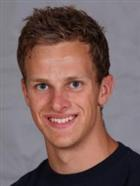
\includegraphics[scale=0.55]{figs/mads.jpeg} \\
	Mads Friis Bornebusch (s123627)\\ [10pt]
		\vspace{0.15cm}
	\end{center}
	\end{minipage}
\end{figure}

\begin{figure}[h!]
	\centering
	\begin{minipage}{0.40\linewidth}
	\begin{center}
	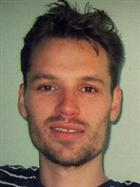
\includegraphics[scale=0.55]{figs/tobias.png} \\
	Tobias Tuxen (s120213)\\[10pt]
		\vspace{0.15cm}
	\end{center}
	\end{minipage}
\end{figure}

\begin{figure}[h!]
	\centering
	\begin{minipage}{0.40\linewidth}
	\begin{center}
	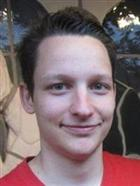
\includegraphics[scale=0.55]{figs/kristian.jpeg} \\
    Kristian Sloth Lauszus (s123808) \\ [10pt]
		\vspace{0.15cm}
	\end{center}
	\end{minipage}
\end{figure}


\vspace*{\stretch{2}}
\end{center}
\begin{flushleft}
\subtitle\\
DTU Space\\
\dato
\end{flushleft}


	
	%%% INDHOLDSFORTEGNELSE OG ABSTRACT %%%
		\chapter{Resumé}

I dette programmeringsprojekt har vi skrevet og designet al koden til spillet Reflex Ball. Koden er skrevet i C i compileren Z8Encore! og implementeret på en Zilog 6403 mircocontroller. \\ \\
Vi har konkluderet at den skrevne kode implementerer det ønskede kredsløb på Mircrocontrolleren, da alle spillets facetter er blevet gennemtestet og giver det ønskede output. Som slutresultat har vi et fuldt funktionelt ReflexBall-spil med mange udvidelser der bl.a. inkluderer brikker (Arkanoid-stil), power-ups, forskellige levels og styring med ret. Der er indtil videre ikke fundet nogle bugs i slutversionen af spillet.\\ \\		
		\chapter{Abstract}

In this programming project we have written and designed all the code to the game Reflex Ball. The code has been written in C in the compiler Z8Encore! and has been implemented on a Zilog 6403 Mircrocontroller. \\ \\
We have concluded that the written code implements the desired circuit on the Microcontroller as as all the different facilities of the game has been thoroughly tested and is in compliance with the expected result. In the end we have a fully functional Reflex Ball Game with many expansions, which amongst others, include bricks (Arkanoid style), power-ups, different levels and steering-wheel game controller. So far no bugs has been found in the final version of the game.

\begin{figure}[h!]
\centering
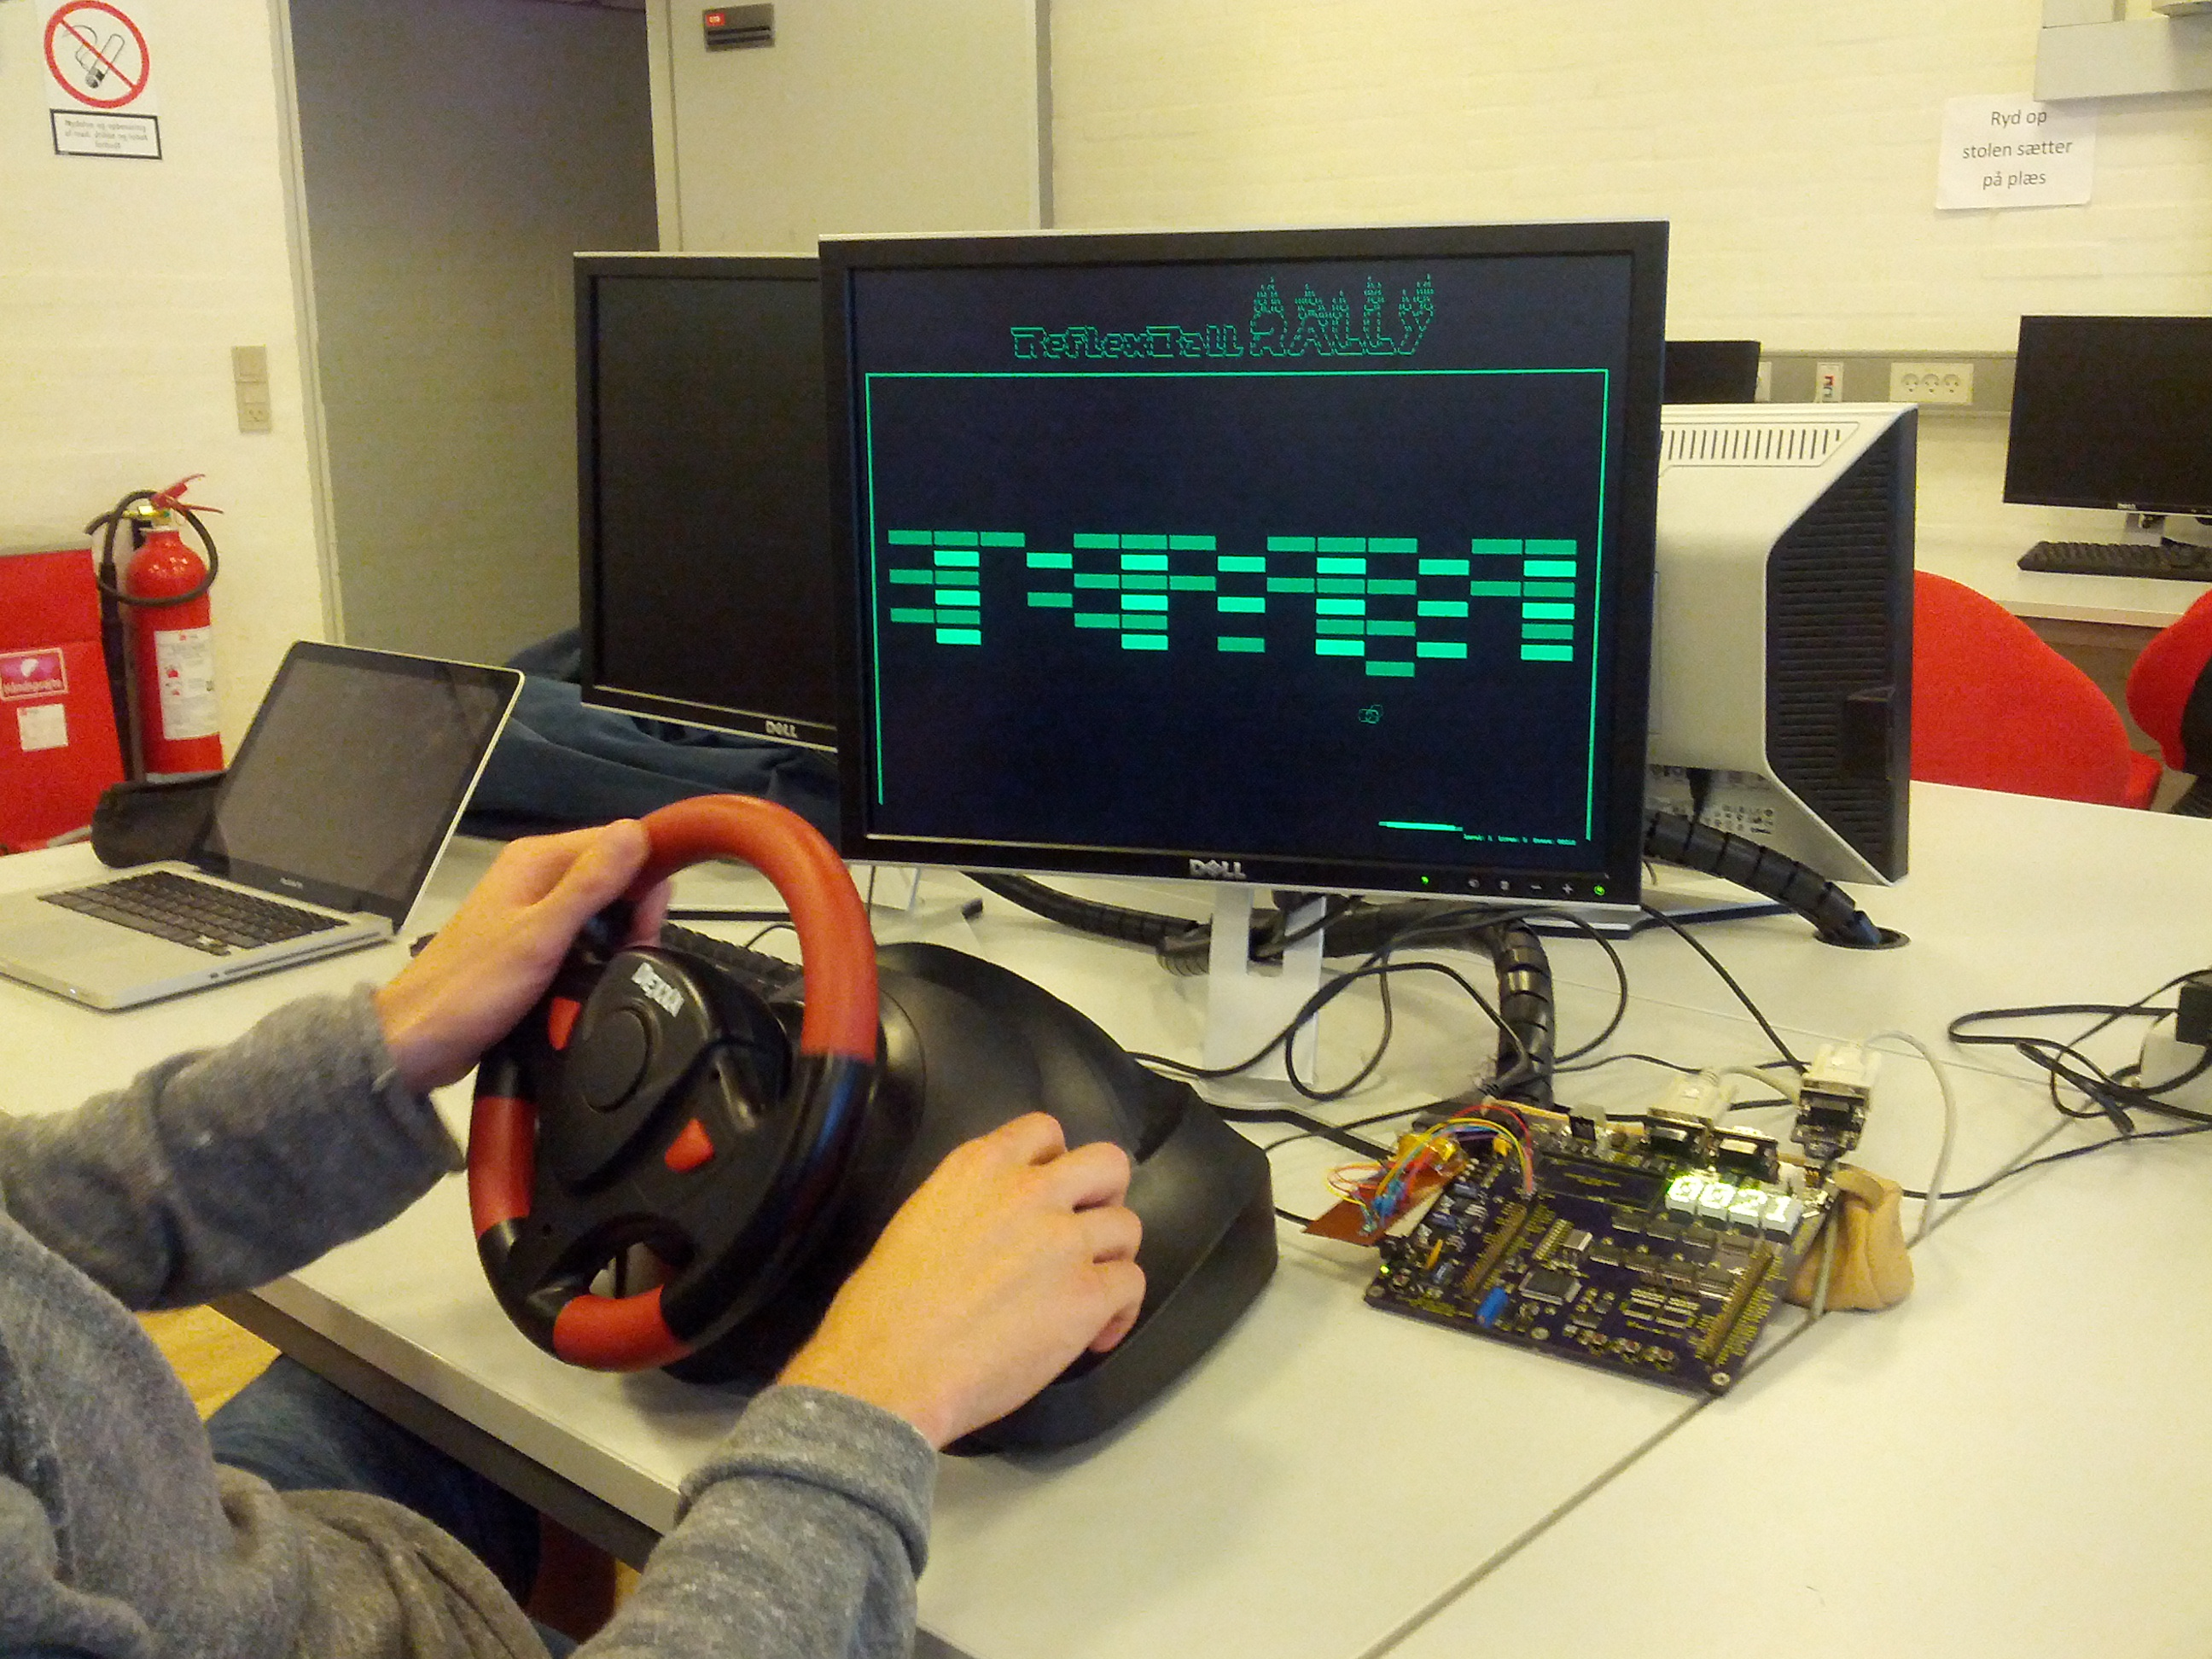
\includegraphics[scale=0.5]{figs/forside.png}
\caption{Screenshot from our implementation of ReflexBall}
\label{fig:awesome}
\end{figure}
		\newpage
		\chapter{Fordord}

Denne rapport er skrevet som en del af eksaminationen i DTU kursus 30010 Programmeringsprojekt. Alle tre, på forsiden nævnte, gruppemedlemmer har bidraget til rapporten på lige vis. Vi har lavet alle forberedelsesøvelser, skrevet koden og afsnittene i rapporten i fællesskab. Denne rapport beskriver vores arbejde og resultater.\\ \\ \\ \\ \\ \\

\begin{figure}[h!]
\centering
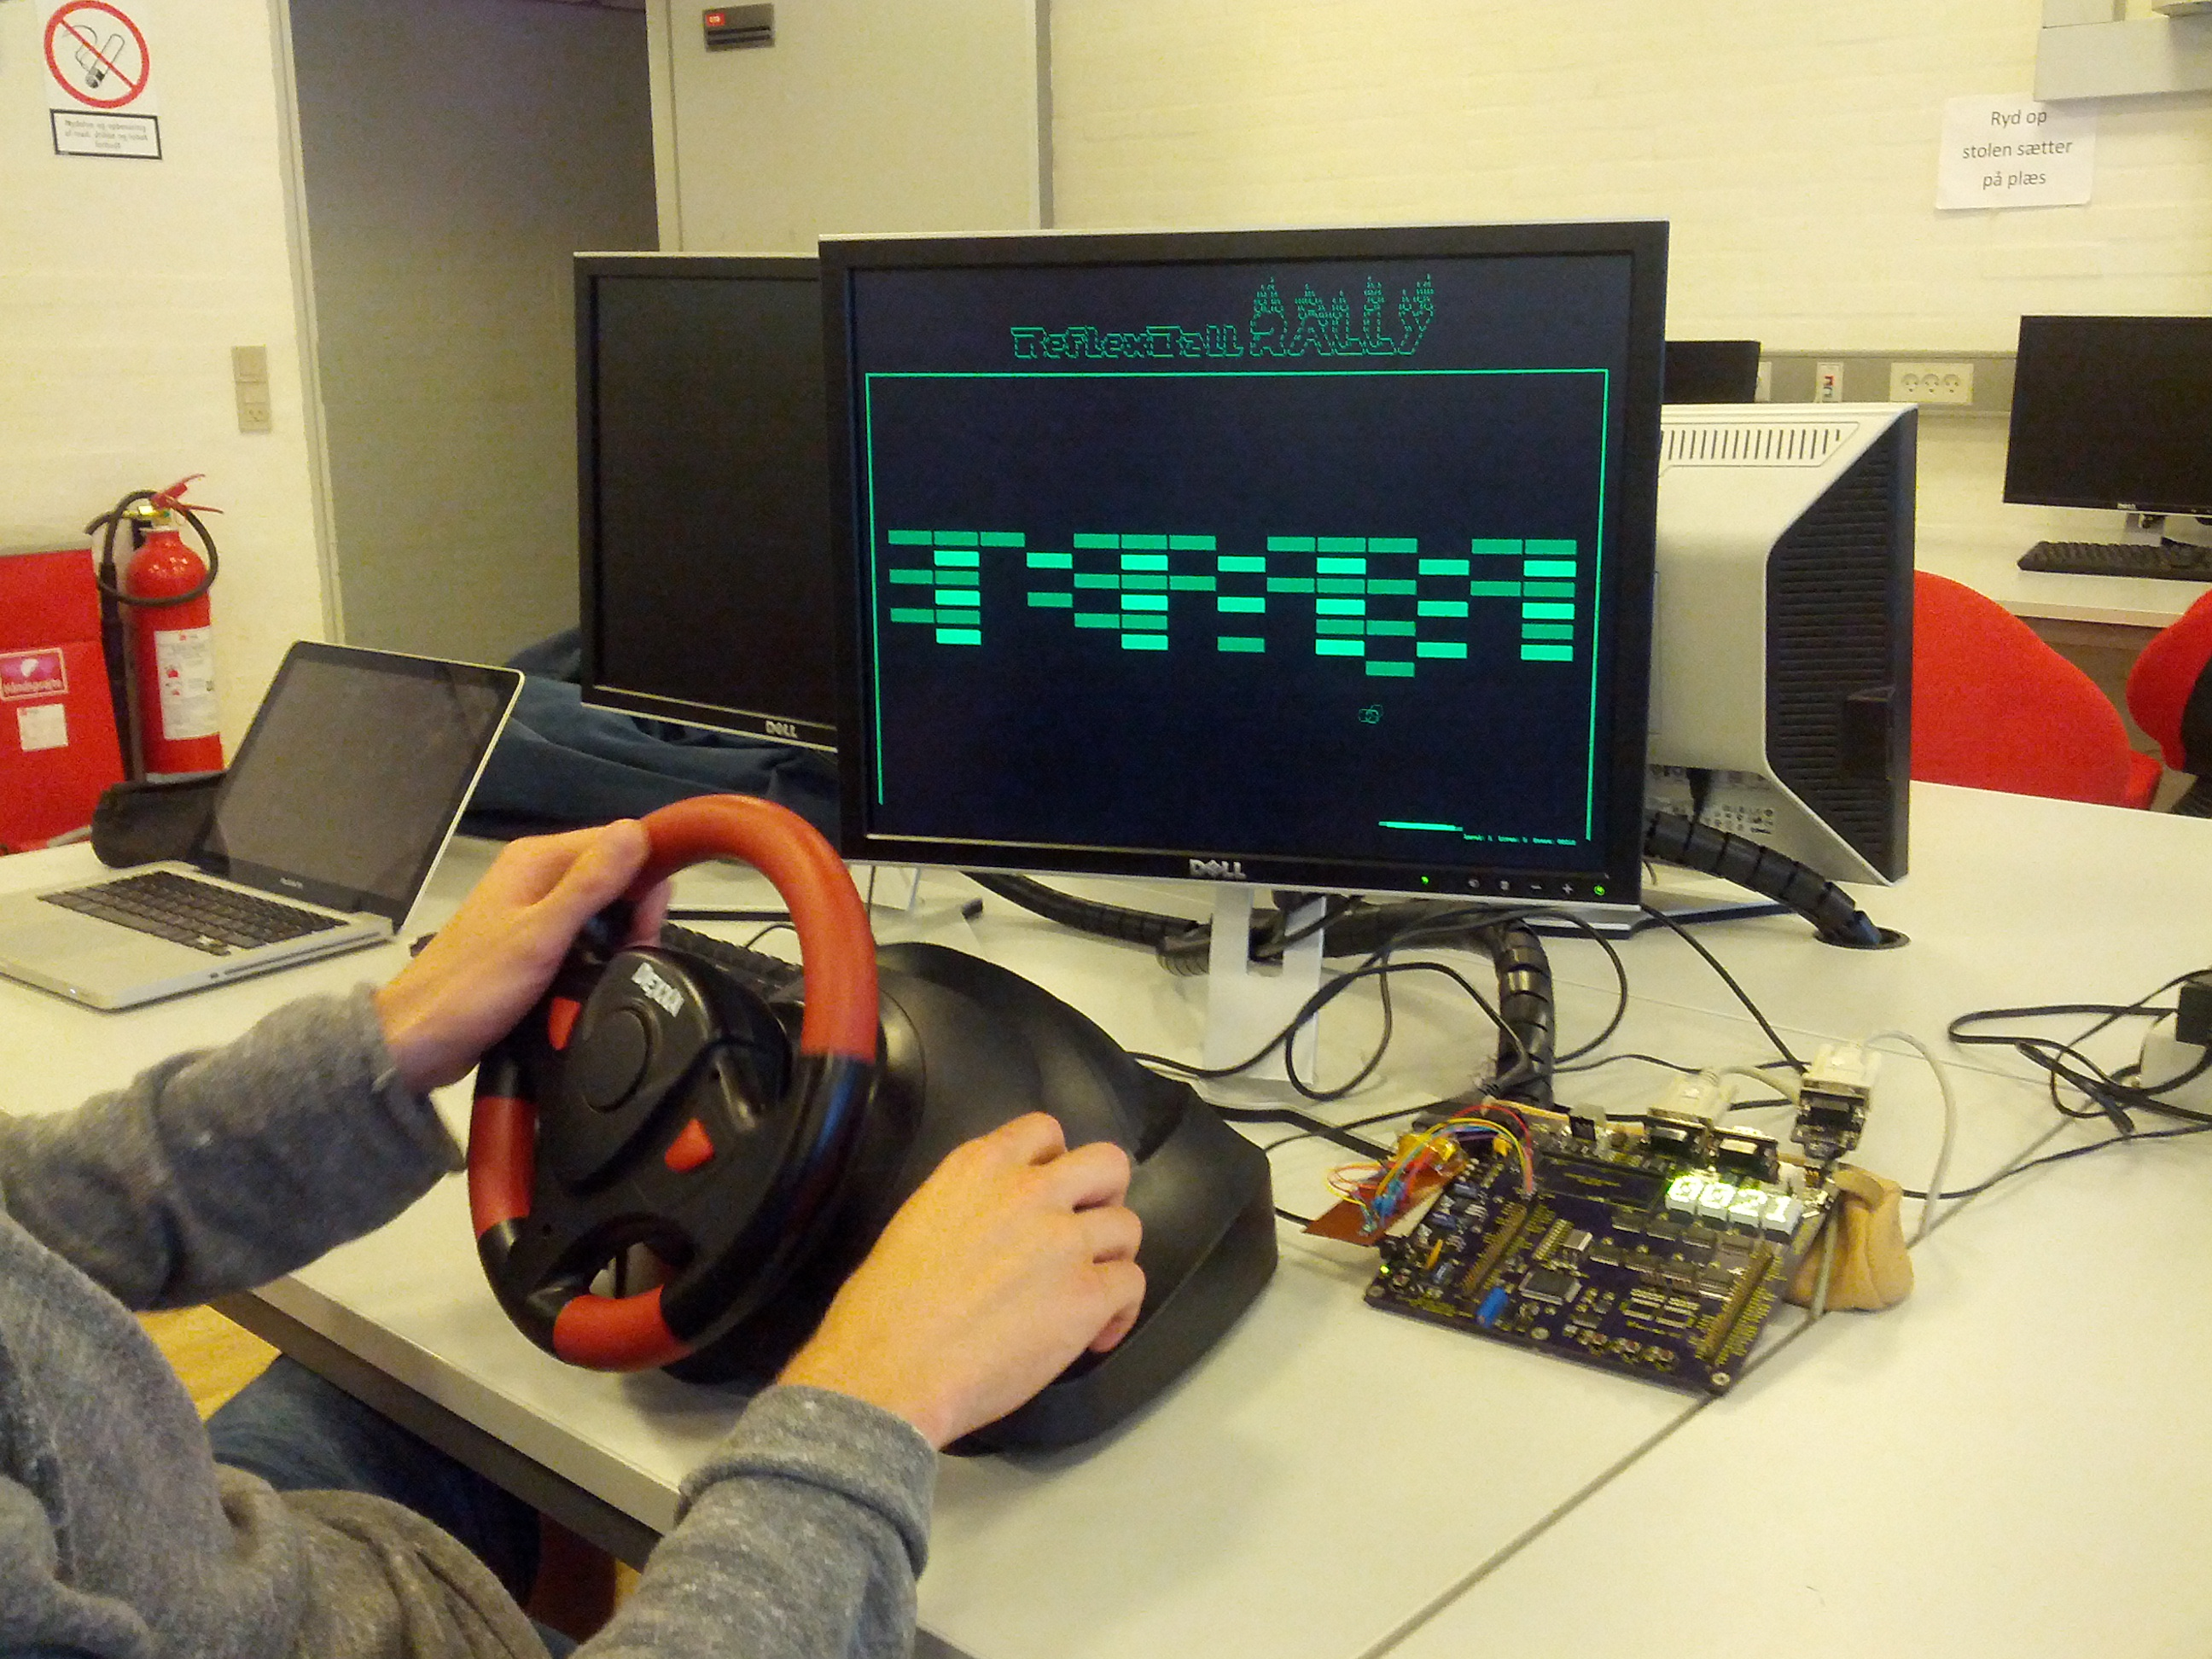
\includegraphics[scale=0.17]{figs/forside.jpg}
\caption{Screenshot from our implementation of ReflexBall}
\label{fig:forside}
\end{figure}
		\newpage
		\tableofcontents*						% Indholdsfortegnelse (fjern * hvis der skal stå "Indhold")
%        \listoffigures*						% Figurliste

		
	%%% RAPPORTINDHOLD %%%
		\mainmatter
%		\input{tex/maple}
		\chapter{Introduktion}

This report documents the design and implementation of the control part of a vending-machine for soft-drinks. \\

The project was divided into three laboratory exercises, in which parts of the system was designed. After the finalization of all three laboratory exercises a complete vending machine control circuit was designed and implemented on a Basys2 FPGA board. The optional parts of the lab exercises is included in the elaboration of each of the exercises, which also redefines some of the mandatory functions, and update/change them as the requirements of each part changes a we move towards the finished control part. \\
		\chapter{Basalt design}
The vending machine should be able to sell only one item at a time, not returning any money. Surplus will be left for next purchase. The price of an item is selected automatically when the user selects a product. The machine only accepts 1, 2 and 5 kr. The price of the selected item is displayed as a two-decimal-value on two seven-segment-displays as will the current sum-available-for-purchase. 

\begin{figure}[h!]
\centering
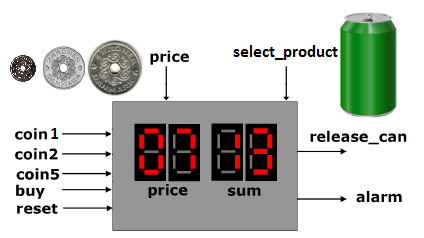
\includegraphics[scale=0.8]{figs/vendingdisplay.png}
\caption{Sketch of the vending machine}
\label{fig:vendingdisplay}
\end{figure}

As seen on figure \ref{fig:vendingdisplay} there is a number of user inputs. coin1, coin2, coin5 and buy is emulated by push-buttons on the FPGA board. The fifth 'input' select\_product, is emulated by switches, which choose between the different types of products, and the prices matching to every type. \\

When a product is chosen by a switch, the name of the product is shown for approximately 1.3 seconds. After this, the price is shown on the two digits to the left. The rightmost two digits represents the sum of the coins 'inserted' by the push-buttons coin1, coin2 and coin5. When the buy button is asserted, the price is subtracted from the sum if sum is greater than or equal to the price of the product. In the case where the sum is lower than the price, an alarm signal wlll be asserted, causing all four digits to blink for a fixed amount of time (approximately 1.3 seconds) on a 3Hz clock. If the 'Reset' switch is asserted, the sum is set to zero while the price of the products persists. \\

In designing the Vending Machine, we have created a number og VHDL entities, each controlling a part of the complete machine. Below is a block-diagram of our VHDL implementation of the machine. 

\begin{figure}[!h]
\centering
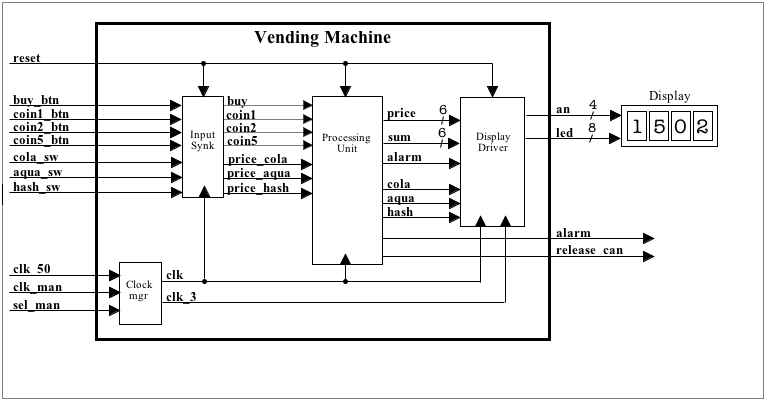
\includegraphics[scale=0.7]{figs/structure.png} 
\caption{The structure of our VHDL design, including the structure, entities and components}
\label{fig:structure}
\end{figure}
		\chapter{Introduktion}

This report documents the design and implementation of the control part of a vending-machine for soft-drinks. \\

The project was divided into three laboratory exercises, in which parts of the system was designed. After the finalization of all three laboratory exercises a complete vending machine control circuit was designed and implemented on a Basys2 FPGA board. The optional parts of the lab exercises is included in the elaboration of each of the exercises, which also redefines some of the mandatory functions, and update/change them as the requirements of each part changes a we move towards the finished control part. \\
		\chapter{Implementation og tests}
\section{Hej Mads}
\section{Hallo}

\subsection{Clock Manager}
In this entity the different clock signals are generated as dividers of the master on-board 50 MHz clock. \\ 
We generate two sub-clocks. One \texttt{clk} that runs at $50000000/(2^16) = 762.94$ Hz. And a slow clock \texttt{clk\_3} for the alarm-blink signal, which runs at $50000000/(2^24) = 2.98$ Hz.

\subsection{Input Synchronization and avoiding metastability}
All the inputs from the outside world must be synchronized to the clock. This is done to avoid meta-stability, which is a very undesirable condition in digital systems. Meta-stability can occur if an input value is changed too close to the clock edge violating either the setup- or holdtime of the gate. If the setup/hold times are violated, there is no way to tell if the input will go low or high, which of course is a problem in itself. The biggest problem however is not the uncertainty of whether the signal goes low or high, but the fact that there's no way of knowing exactly how long the value will be afloat between low and high. It is only possible to give probabilities of how long a metastable state will last. An example of metastability in practice can be seen on figure \ref{fig:meta}, where several experiments shows the uncertainty of the whether the signal is going high or low an more importantly the uncertainty of how long the metastable state lasts.\\

\begin{figure}[!h]
\centering
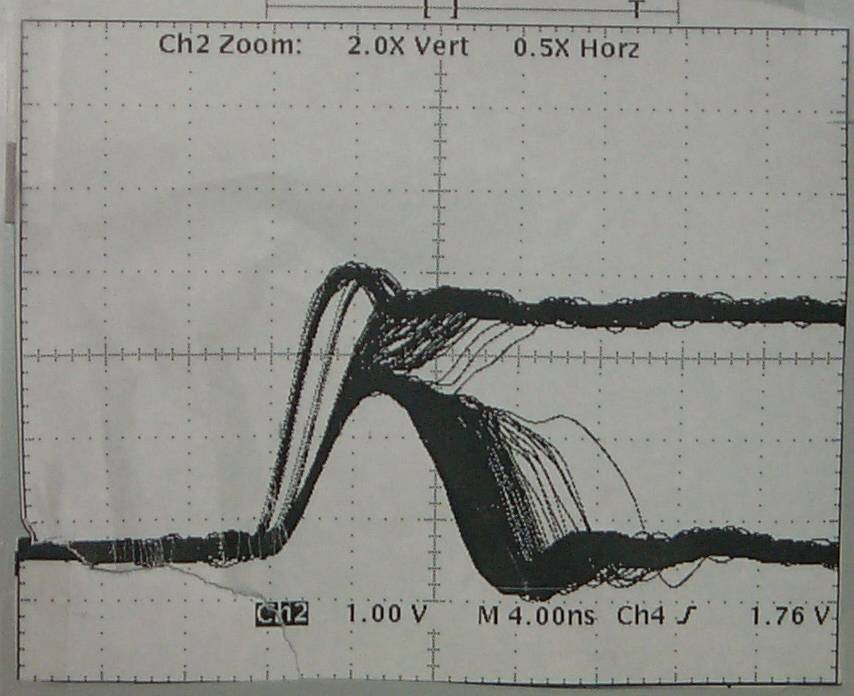
\includegraphics[scale=0.3]{figs/meta_pic.jpg} 
\caption{A practical example of metastability}
\label{fig:meta}
\end{figure}

Synchronization is generally done by passing the input value into one or more flip-flop's which is synchronized to the clock. Some signals in our design (\texttt{coin1}, \texttt{coin2}, \texttt{coin5} and \texttt{buy}) not only need to be synchronized with the clock, but also need their pass-on signal to be activated for exactly one clock cycle only. This is due to the fact that even though you press a button for only as short a while as you are able to, the clock still ticks at about 760Hz which, in almost every situation, will lead to an active input for several clock cycles. This 1-clockcycle-active is done by running the signal through 2 consecutive flip-flops and only letting the pass-on signal go high as long as the output of the first flip-flop is high and the output from the second flip-flop is low. In order to get the pass-on signal activated again, the input signal needs to be turned off first. 

\subsection{Implementing the display-driver}
To begin with as a part of the lab-exercises in this course we implemented the display-driver as a 'Hexadecimal to seven-segment display' state machine, having one state per possible hexadecimal. This was implemented as a Process in VHDL. When the 4-bit binary input \texttt{d} changes value (see Appendix A - display\_driver), the LED's of the display reflects the change.\\

\begin{figure}[!h]
\centering

\includegraphics[scale=0.5]{figs/single_digit_1.png} 
\caption{The representation of the 4-bit binary value "0001"}
\label{fig:single_digit_1}
\end{figure}

In order to display hex-numbers on a seven-segment display, we have build a combinational circuit in VHDL to convert a 4-bit binary number into the patterns which represent the number on a single seven-segment display. \\

There is no clever logic between the input and output in this case, since the LED's needed to display the different characters have no logical relation to the value that needs to be on the display. 
Therefore the implementation is a direct implementation of the state-table. \\

We implemented our state-table in a \texttt{Process(d)}. The input signal \texttt{d} is represented as an \texttt{UNSIGNED} 4-bit-vector. This process has a nested case statement, which represents the truth table. \\

The signal \texttt{led} is an \texttt{UNSIGNED} 8-bit-vector, 7-bits for the lines and one for the dot. \\

In this frame the first two lines of the \texttt{Process(d)} is show.
\begin{framed}
\texttt{
Case d IS \\
	WHEN "00000" => led <= NOT "11111100"; -- 0 \\
	WHEN "00001" => led <= NOT "01100000"; -- 1 \\
}
\end{framed}

\subsubsection{Expanding design to binary-coded-decimal instead of hexadecimal}
This hex-design was quickly abandoned, as it is not practical to read a price-tag in hexadecimal. Therefore we expanded our design to display binary-coded-decimal (BCD) values on the display instead. \\

The seven-segment logic was left untouched as the displays still must be able to display the numbers from 0-9, the hex-decimal-states was left untouched but is not used in our design. Later the state table was expanded further to enable us to display the characters needed for the displaying of product-names. See appendix A, figure \ref{vhd:dispdriv1}.

The input word \texttt{(d)} was changed from a 4-bit \texttt{UNSIGNED} to a 5-bit \texttt{UNSIGNED}. \texttt{d} had to be expanded to make room for the ekstra characters needed for the product names.

Further more the input values to display \texttt{price} 
This allows the two 2-decimal displays (price \& sum) to display values between 0-63.

\subsubsection{Time multiplexing the four seven-segment-displays}
To enable the displays to represent four different values to the user time multiplexing was implemented. Time multiplexing means cycling through the displays, turning them on one by one and displaying the corresponding value on the target display. \\

This is implemented by a 2-bit counter, incremented by the rising\_edge of the clock. The 2-bit overflow makes sure that the counter-value \texttt{m} stays between 0-3. The counter is incremented like so: \texttt{m\_next <= m + 1}. This counter is used a the selector to a multiplexer, selecting the right value for the corresponding display. The counter-value \texttt{m} also controls which display-anode \texttt{(an)} is turned on. Thus, each display is only turned on when it's value is represented on the 8-bit \texttt{led}-vector.

\subsection{Implementing the Processing Unit}

The Processing Unit is the central arithmetic core unit of the vending machine. This component calculates the total amount of coins inserted, and determines whether or not enough coins are inserted to purchase a product and if this is the case, subtracts the product of price from the total amount inserted. The Processing Unit is also the component taking care of asserting an alarm signal if a buy is attempted with too low total coin amount inserted as well as setting a the price and displaying the product name when a product is chosen. Below it is explained how the Processing Unit operates when one of the four different types of inputs are asserted:

\begin{itemize}
\item If \texttt{Reset} is asserted the sum will be set to zero.
\item If one of the three \texttt{price\_product} signal are asserted the \texttt{product} signal will be set to 1 for limited time period. This will cause the \texttt{price\_out} signal to be set to the value of the product as well as displaying the name of the product on the LEDs for as long as \texttt{product} is 1.
\item If one of the three \texttt{coin} input signal are asserted the Processing Unit will cause the sum signal to be incremented by the value of the coin inserted.
\item If the \texttt{buy} input is asserted, the machine will calculate whether buy is greater than or equal to price. If this is the case a \texttt{release\_can} signal is set to 1 and the price is subtracted from the sum. Notice that the \texttt{sum} signal won't be set to zero after a successful buy, because the machine is designed in such a way that it doesn't give back money (a good business design!). On the other hand if the \texttt{buy} input is asserted when sum is less than price, the alarm signal will be set to 1 for a limited amount of time, causing the display to blink on a 3 Hz clock for a approximately a couple of seconds. Notice here that the alarm counter \texttt{alarm\_count} runs on the normal 763 Hz clock and therefore the alarm signal is not synchronized to the 3 Hz clock, meaning that the alarm signal can start and stop in the middle of a 3 Hz clock period.
\end{itemize}

In the \texttt{process(coin1, coin2, coin5, buy, clock)}, we have chosen nested if else statements so that Reset have highest precedence, then the coins, then alarm and finally buy. It's obvious that we want Reset to overrule all other inputs, but the coin inputs have higher precedence than alarm as you would always want a machine to register when coins are inserted even though the alarm is on (unless you a mean business man!). buy however has lower precedence than alarm, as we want the machine to stop alarming (aka blinking) before another buy can be attempted. \\

To test whether the written VHDL code for this component works as intended, we simulate it in the ModelSim environment. This is done by writing a .do file for ModelSim, which sets the input signals to relevant combinations, and simulating clock signals. By doing this it is tested if the output signals are as intended. The .do file can be seen in figure \ref{fig:dofile}.

\begin{figure}[h!]
\centering
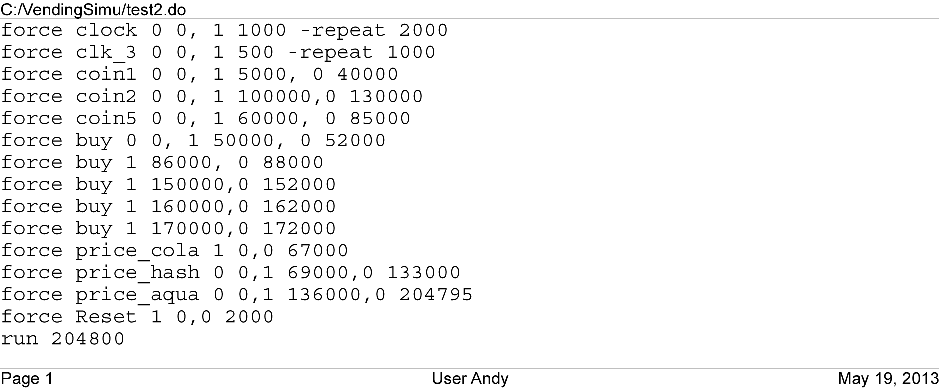
\includegraphics[scale=0.8]{figs/dofile.pdf}
\caption{Do-file for the Processing Unit ModelSim simulation}
\label{fig:dofile}
\end{figure}

The timing diagram in figure \ref{fig:simu}. is imported from ModelSim and shows the simulated components response to different inputs. As expected the \texttt{price\_out} changes to the wanted value when a product signal is switched on. It is also seen that \texttt{cola\_out}, \texttt{hash\_out} and \texttt{aqua\_out} respectively is set to 1 when the when the price switch for each of the products is asserted. This is the signal which are passed on to the display driver, which writes the product name on the display. Since the name is set to be there for approximately 2 seconds, this simulation does not show that these -\texttt{\_out} signal are de-asserted after this period of time, since the simulation only cover 0.002 s, even though the simulation clock ticks faster. It is also seen that the calculating mechanism works correctly since the price is subtracted from the sum and yields the correct value, when buy is asserted. It is seen as well that the \texttt{alarm\_out} signal is asserted (in the last case where price is higher than sum) exactly as it should. It should be remembered that these signals have not been through the input synchronizer which ensure that coin, buy and price signals only are set to one for a single clock period when activated on the Basys board.

\begin{figure}[h!]
\centering
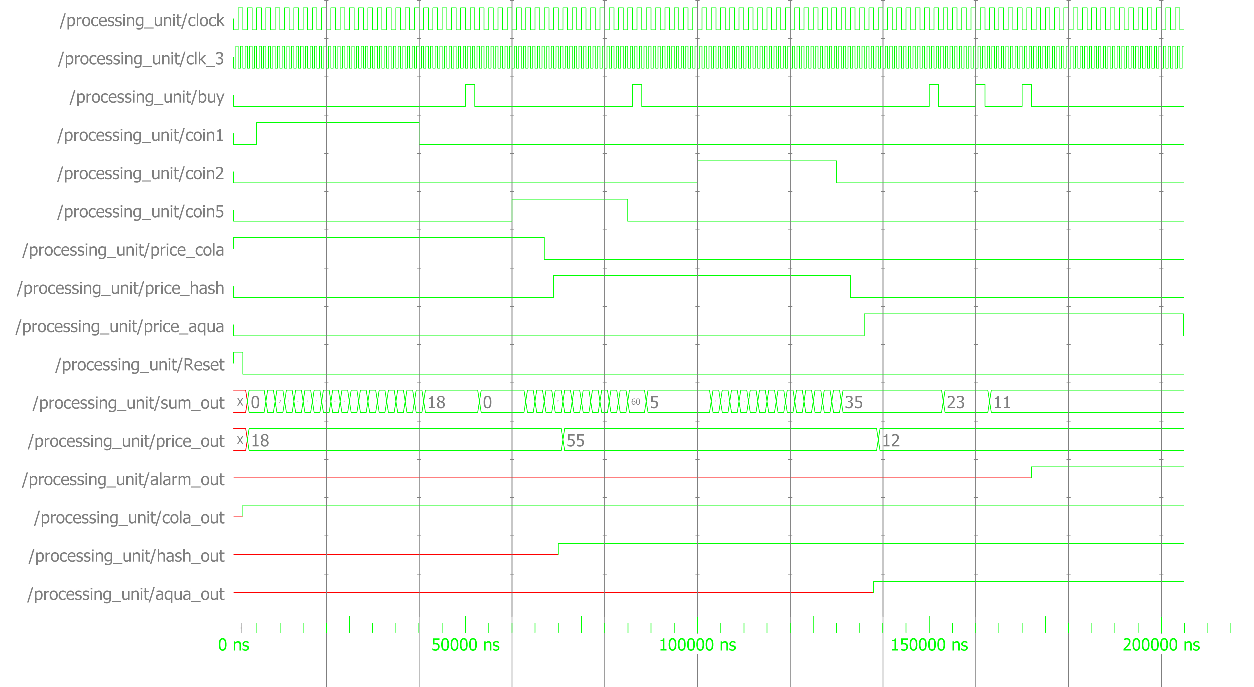
\includegraphics[scale=0.8]{figs/processingunit.pdf}
\caption{Timing Diagram for the ModelSim simulation}
\label{fig:simu}
\end{figure}

\subsection{The structure of the Vending Machine}

The overall structure of the vending machine can be seen in vending\_machine.vhd-file. Here the signals of the different components are tied together to the overall basys-board input and output signals. The components included in vending\_machine.vhd includes the clock\_manager.vhd, display\_driver.vhd, input\_synchronizer.vhd and processing\_unit.vhd \\

Generally the overall structure is that the input signals from the Basys board are connected to the input\_synchronizer to make the signal go high for only one clock cycle when one of the switches or buttons are asserted. Next the signals are sent to the processing unit to compute sum, price, alarm and so on and then finally to display\_driver where the signals are connected back to the Basys board.\\

\begin{figure}[h!]
\centering
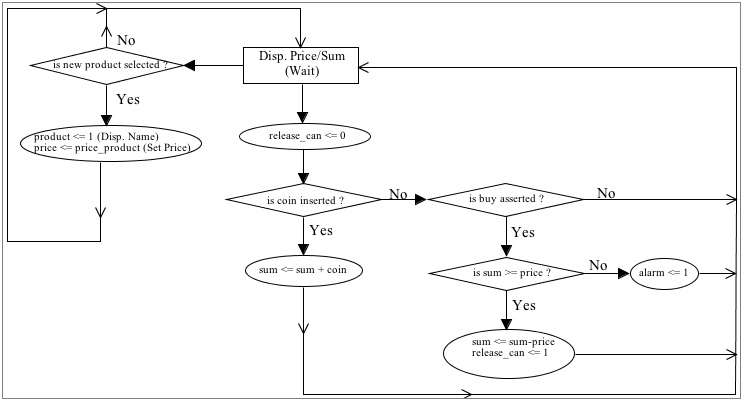
\includegraphics[scale=0.6]{figs/asm_chart.png}
\caption{ASM-Chart showing the overall functionality of the vending machine}
\label{fig:asm}
\end{figure}

On figure \ref{fig:asm} the overall functionality of the Vending Machine is displayed as an ASM-Chart. The machine has 'wait' state where price and sum is displayed. The machine will remain in this state until either a coin is inserted, a product is selected or a buy is attempted. If a product is selected, the product name will be displayed and a the price of that specific product will be set. If a coin is inserted sum will be incremented by the coins value. If buy is asserted and sum is less than price, the alarm signal will be set to 1 causing the both price and sum on the display to blink for a while. If sum is greater than or equal to price, the release\_can signal is set to 1 and sum is subtracted the value of that specific product.
		\newpage
\chapter{Resultater}

In the end we have designed, tested and implemented following components:

\begin{itemize}
\item A clock\_manager with an addition of 3 Hz clock \texttt{clk\_3} 
\item An input\_synchronizer, to synchronize signals from the outside world to the clock, to avoid meta-stability and ensure that some of the signals only goes high for one clock cycle only. This includes buy\_out, coin1\_out, coin2\_out and coin5\_out, cola\_out, hash\_out and aqua\_out.
\item A display\_driver to convert and display price, reset, alarm, sum, cola, hash and aqua-signals on the LED-displays
\item A processing\_unit to calculate the total amount of coins inserted, comparing price with sum when buy is asserted, and either asserting alarm if sum < price, or subtracting price from sum if sum $\geq$ price. The processing unit also passes on the signals which assert product text on the led display, when a product type is chosen.
\item An overall structural component which connects all of the above mentioned components with the in- and outputs on the Basys board.
\end{itemize}














		\newpage
\chapter{Diskussion}
In this section we briefly discuss some of the design choises we have made as well as some expansions we have included in design and finally ideas for further improvements.\\

Below some of the minor modifications we have made in comparison with the design given in the assignment is shown.

\begin{itemize}
\item the release\_can signal has been removed from the code as it doesn't have any real function and therefore, in our opinion, only serves to make the code more confusing. In a practical situation it would be a very quick operation to re-add the release\_can signal.

\item Added coin1 signal which as the name implies is a coin value of 1. we felt this was a logic expansion as most people have 1kr. coins in their purse. As coin1 is placed on one of the buttons on the Basys Board, Reset is instead put on a switch.
\end{itemize}

In our design of the vending machine we have included the following bigger modifications (expansions).

\begin{itemize}
\item Decimal display instead of Hexadecimal display. This is done for both the price and sum outputs displayed on the LEDs. The conversion from a bit-vector to decimal is done with a BCD in the display\_driver.

\item Blink on the display when the alarm signal is asserted. This will cause all both sum and price to blink on a 3Hz clock. The 3Hz clock is made by clock dividing the 763Hz clock display in the clock\_manager.

\item Product names on LED display. When a product is chosen it's name is being displayed for approximately 2 seconds on the LEDs. All others operations can still be done while the product is displayed.

\item Different products to choose from. This includes the 3 products being cola, aqua and hash. These products have different prices which are set when a product is chosen. Choosing a new product will not reset the sum (the total coin amount inserted).
\end{itemize}

Having designed the circuit with the expansions that we wanted, there is especially one idea that we had to leave unimplemented.\\

When designing the machine we felt one aspect missing was making the machine able to repay the left-over coin amount when a product is purchased with a cash\_out signal. A good way to implement this would be to integer divide the left-over amount with 5 then divide the left-over from this division with 2 and finally divide with 1. In this way it is known how many 5-coins, how many 2-coins and how many 1-coins should be payed back to the user. We find that paying the customers back with these coin amounts makes sense as the machine is running on them and therefore seldomly runs out of them. We have chosen not to implement this an expansion however, as we have no place to send these coin values to. We could of course try to display the cash\_out as sentences on the display, telling the customer how many coins of which amounts was returned, but then again it is hard to write on the seven-segment displays as many letters (like M) cannot be displayed on them properly.

		\newpage
\chapter{Konklusion}
Efter spillet et blevet designet, skrevet og uploadet til Zilog 6403 microcontrolleren, er alle spillets facetter blevet gennemtestet og fundet i overensstemmelse med det forventede resultat. Vi kan derfor konkludere at den skrevne kode implementerer spillet Reflex Ball på microcontrolleren og i hyperterminalen korrekt i forhold til specifikationskravene. Derudover kan vi også konkludere at alle udvidelse virker som forventet. \\


		
	%%%	Appendix %%%		
		\newpage\appendix
		\chapter{Appendiks 1}

This appendix contains the complete VHDL-code used, and written/modified by us
%%CLOCK MANAGER

\begin{figure}[h!]
\centering
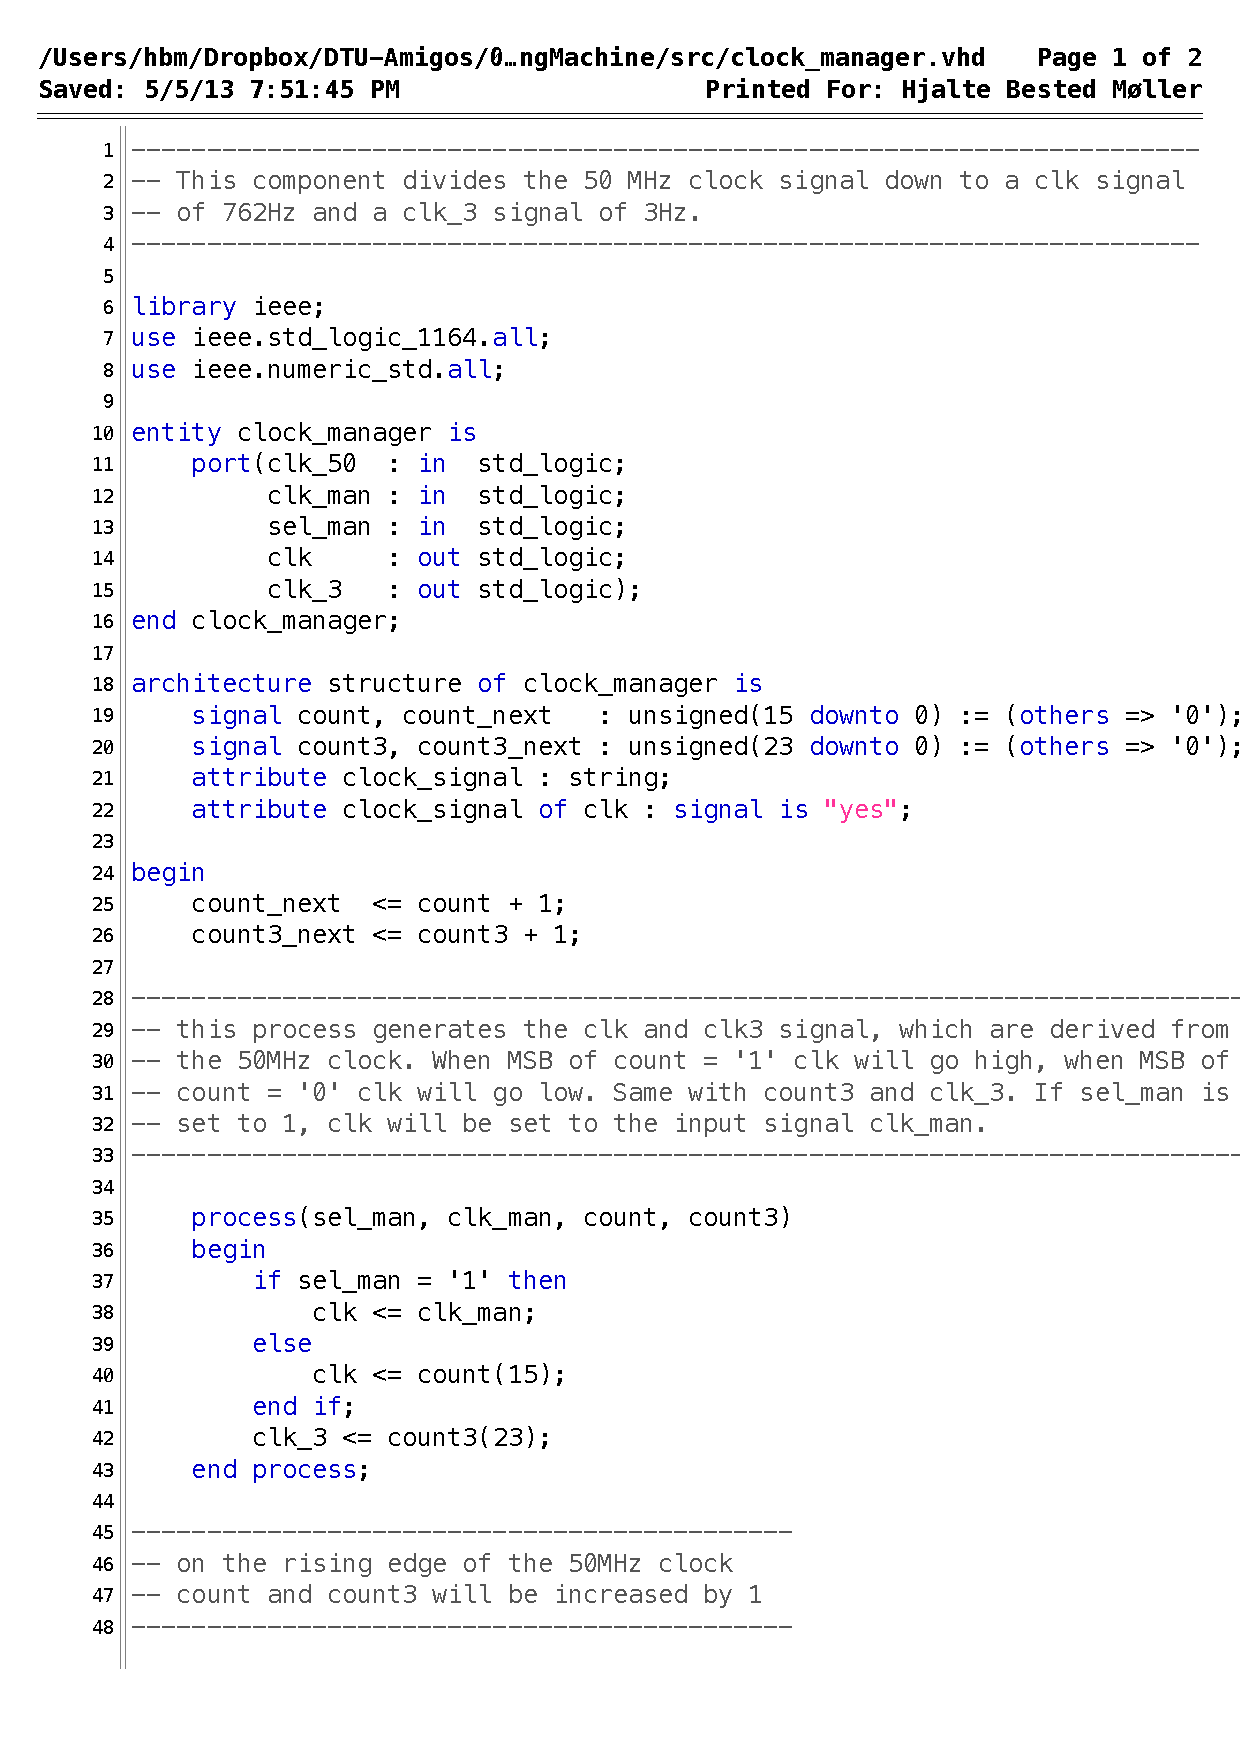
\includegraphics[scale=0.7]{figs/clock_manager.pdf} 
\caption{The clock manager, include our own 3 Hz clock for use in the alarm signal}
\label{vhd:clockman1}
\end{figure}

\begin{figure}[!h]
\centering
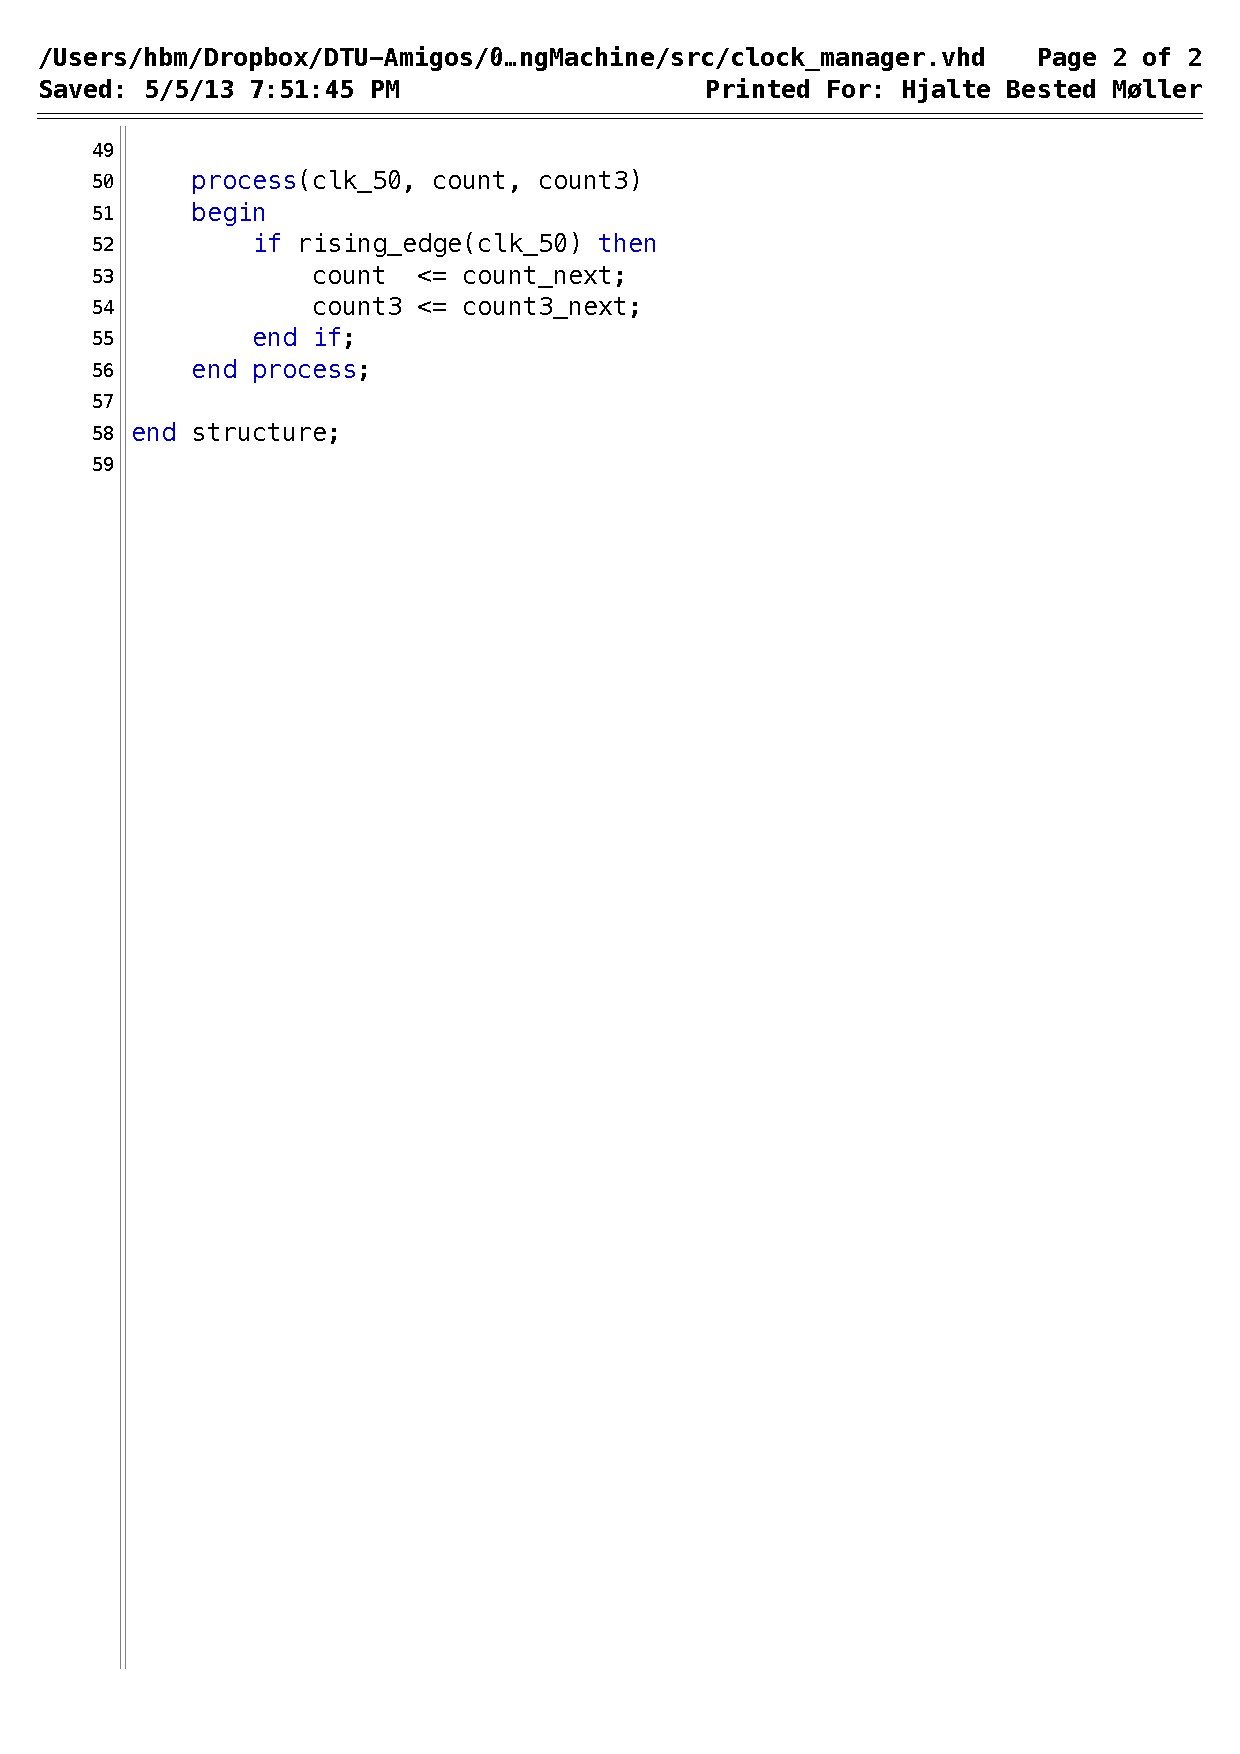
\includegraphics[scale=0.7]{figs/clock_manager_2.pdf} 
\caption{Page 2}
\label{vhd:clockman2}
\end{figure}

%CLOCK MANAGER END

%DISPLAY DRIVER

\begin{figure}[!h]
\centering
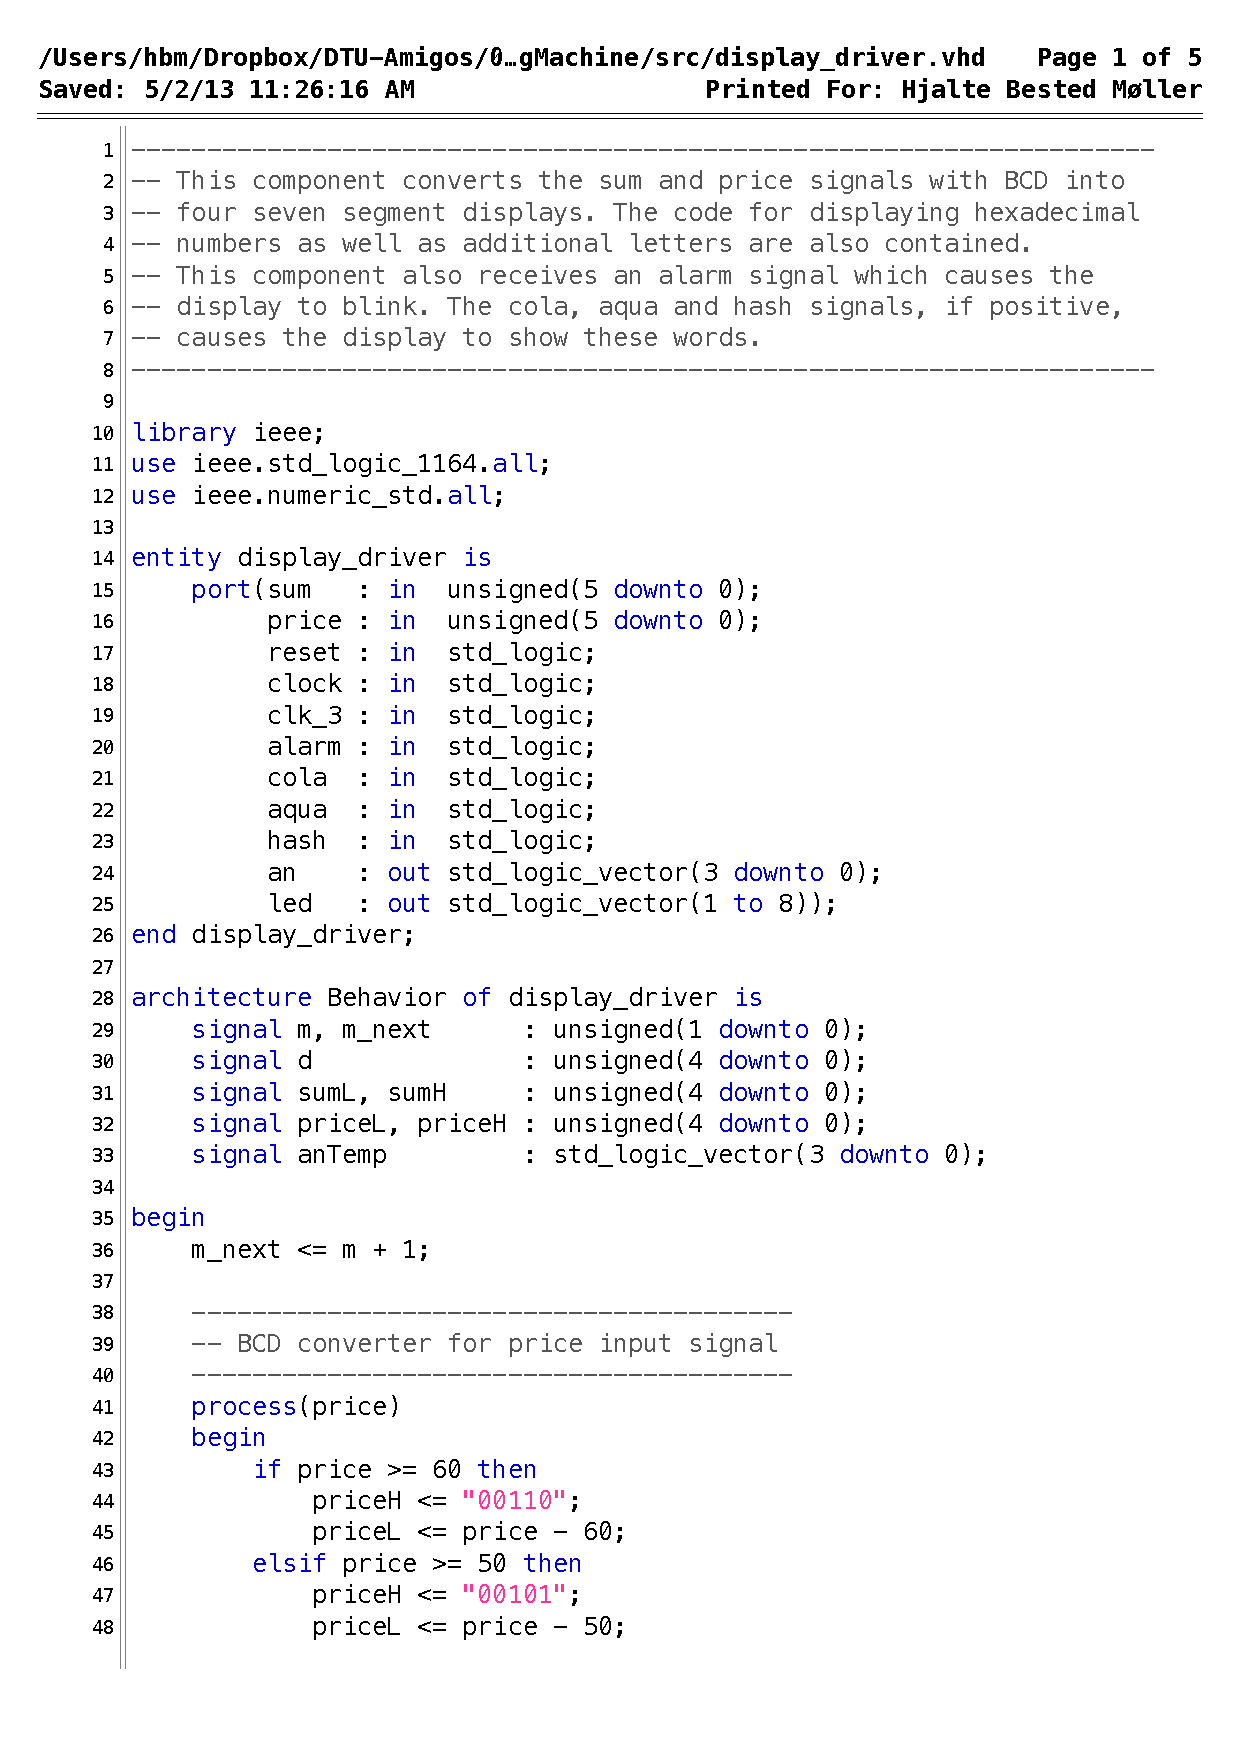
\includegraphics[scale=0.7]{figs/display_driver.pdf}
\caption{Display driver for displaying symbols/numbers on each of the four seven segment displays}
\label{vhd:dispdriv1}
\end{figure}

\begin{figure}[!h]
\centering
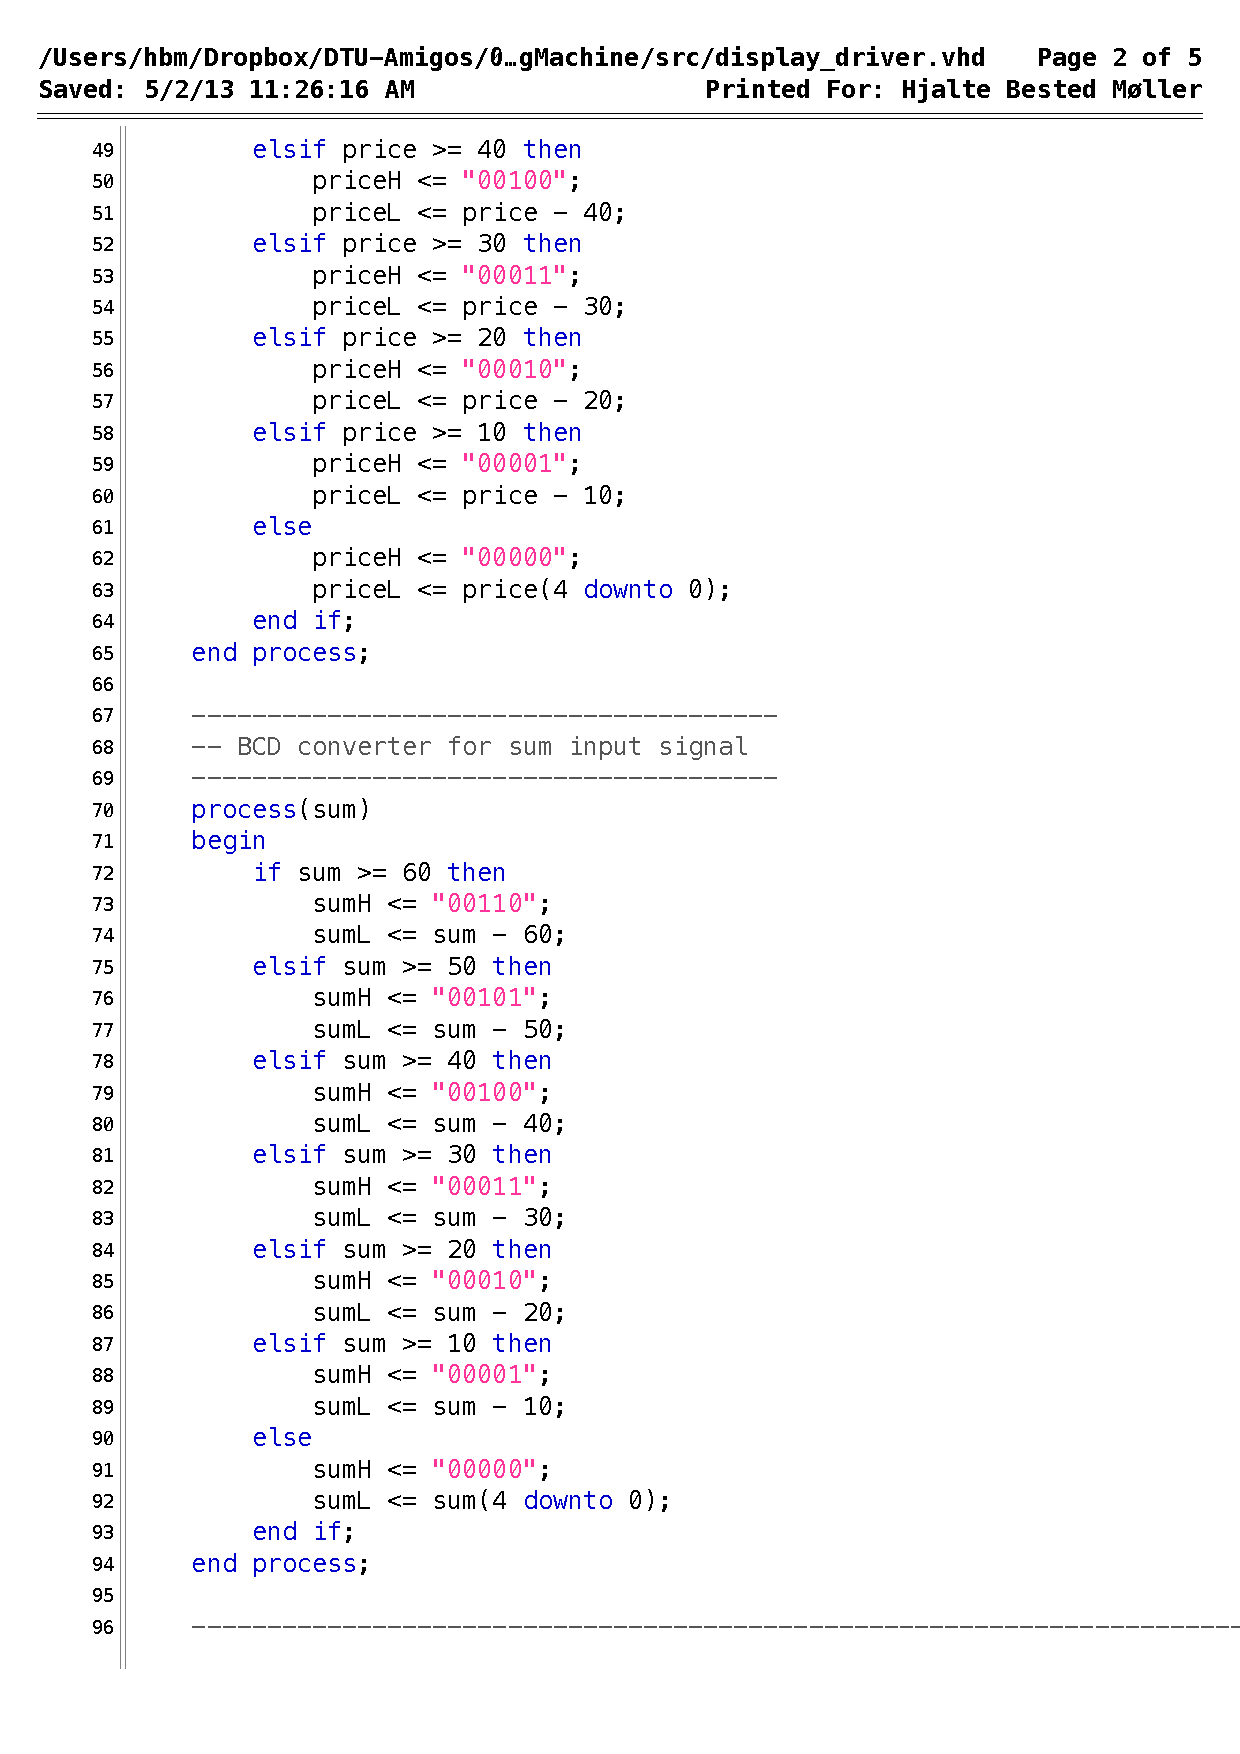
\includegraphics[scale=0.7]{figs/display_driver_2.pdf}
\caption{Page 2}
\label{vhd:dispdriv2}
\end{figure}

\begin{figure}[!h]
\centering
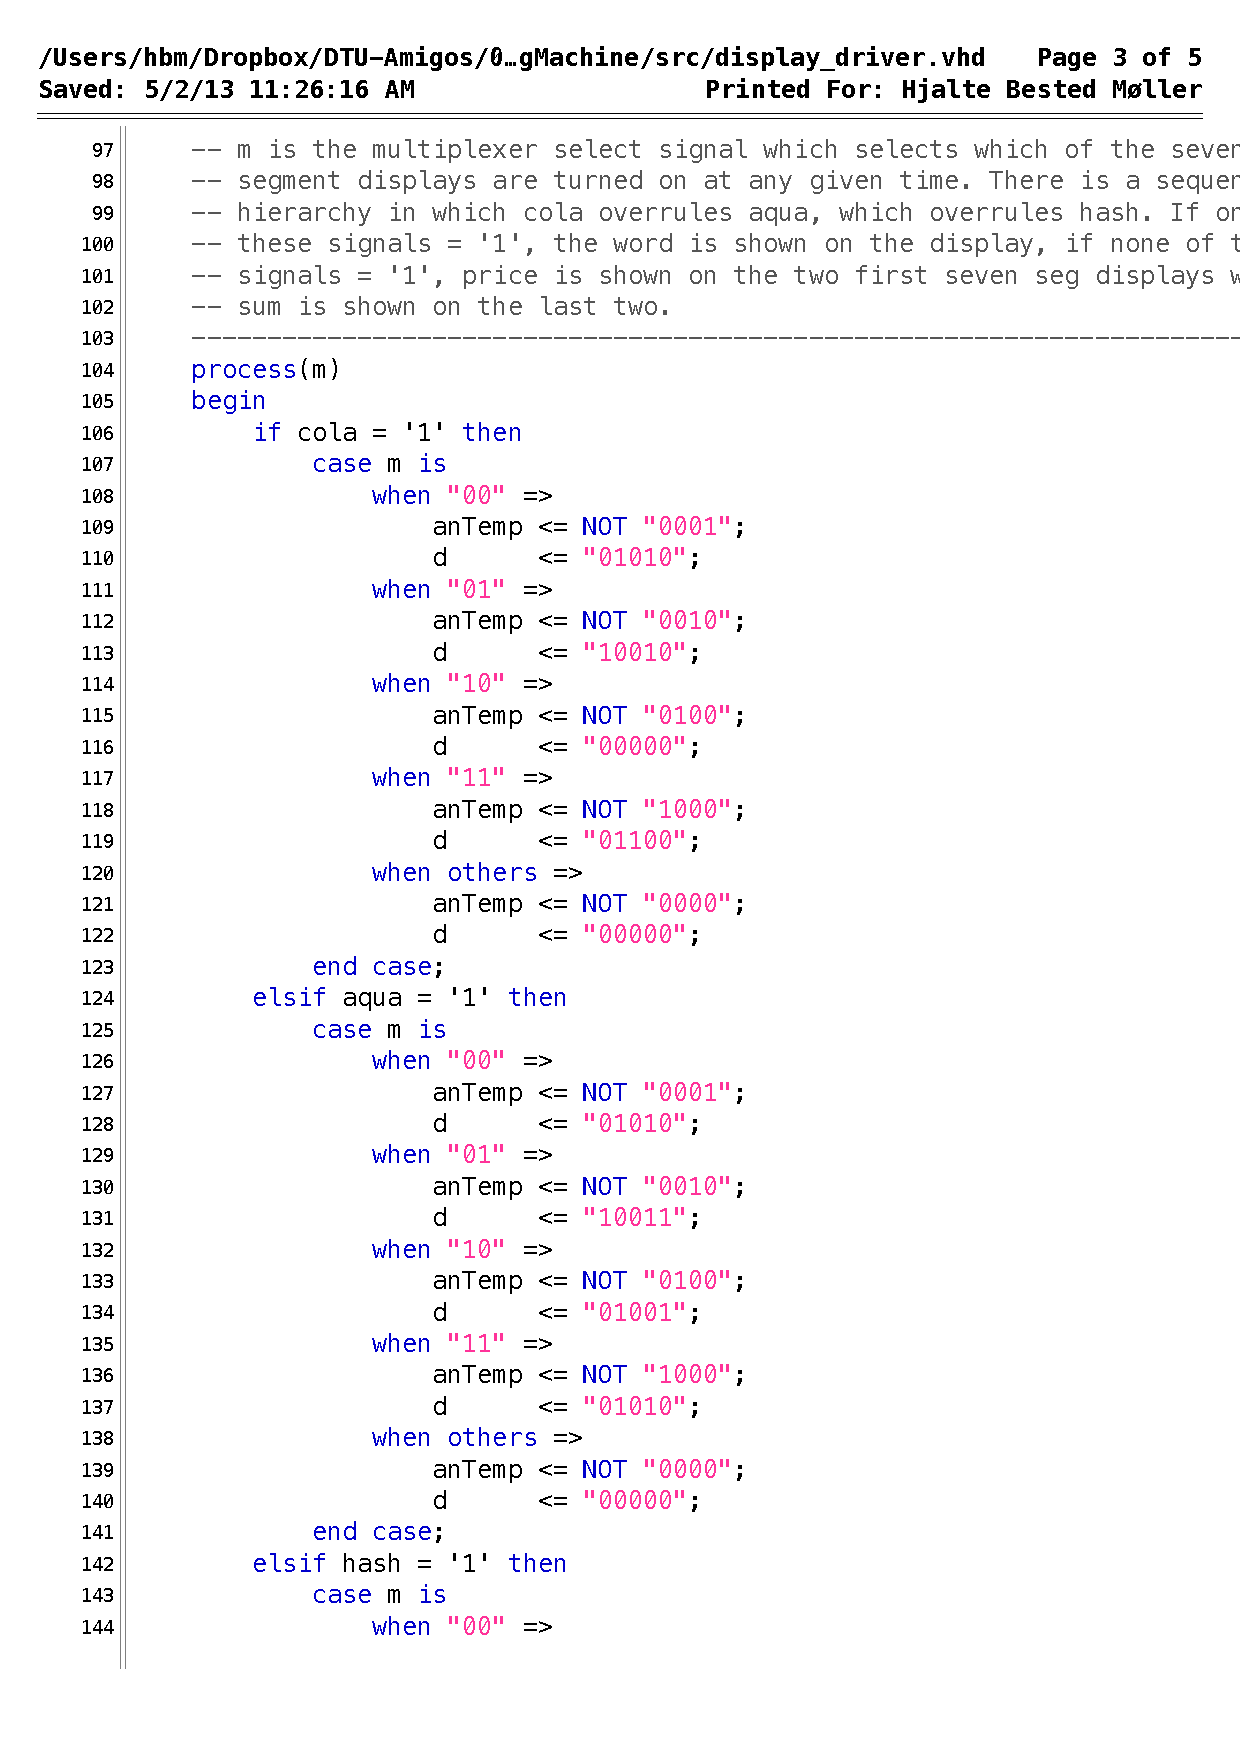
\includegraphics[scale=0.7]{figs/display_driver_3.pdf}
\caption{Page 3}
\label{vhd:dispdriv3}
\end{figure}

\begin{figure}[!h]
\centering
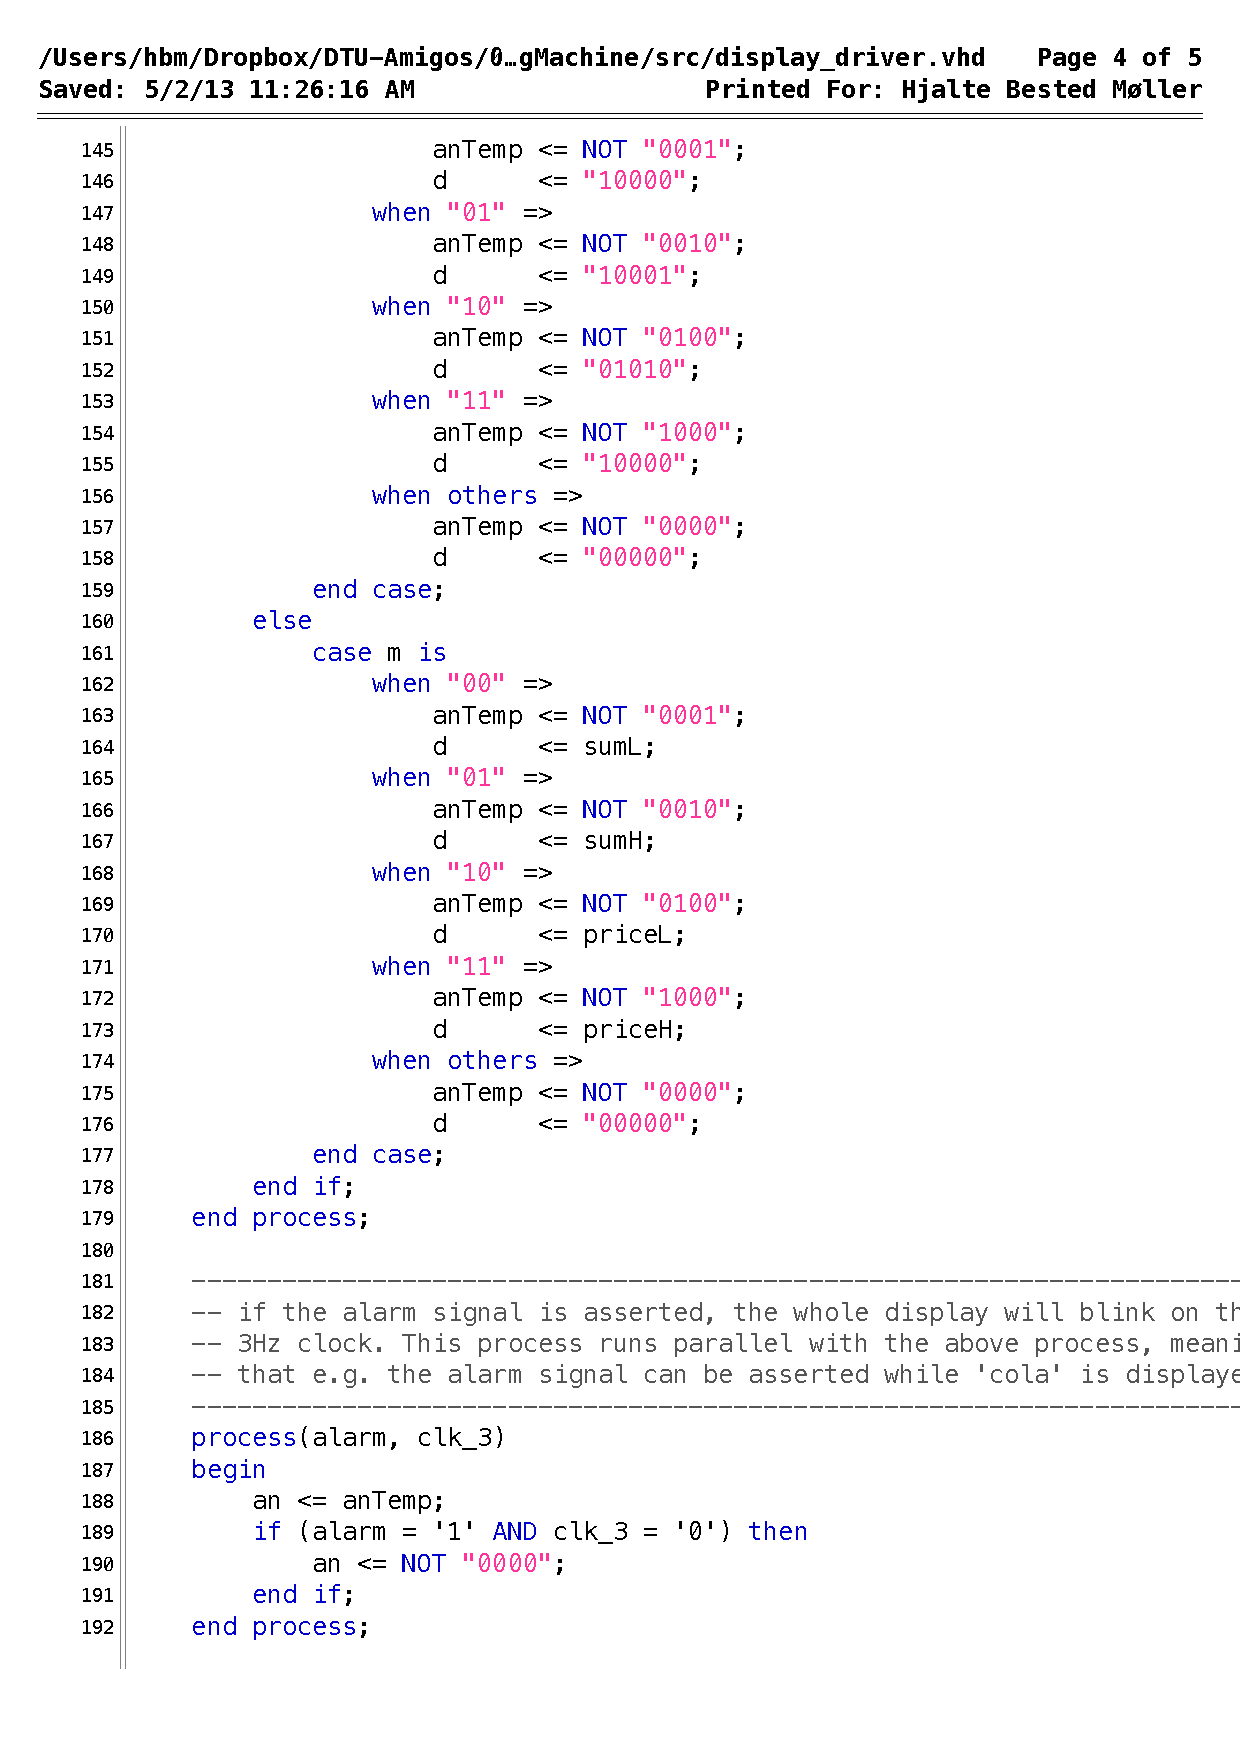
\includegraphics[scale=0.7]{figs/display_driver_4.pdf}
\caption{Page 4}
\label{vhd:dispdriv4}
\end{figure}

\begin{figure}[!h]
\centering
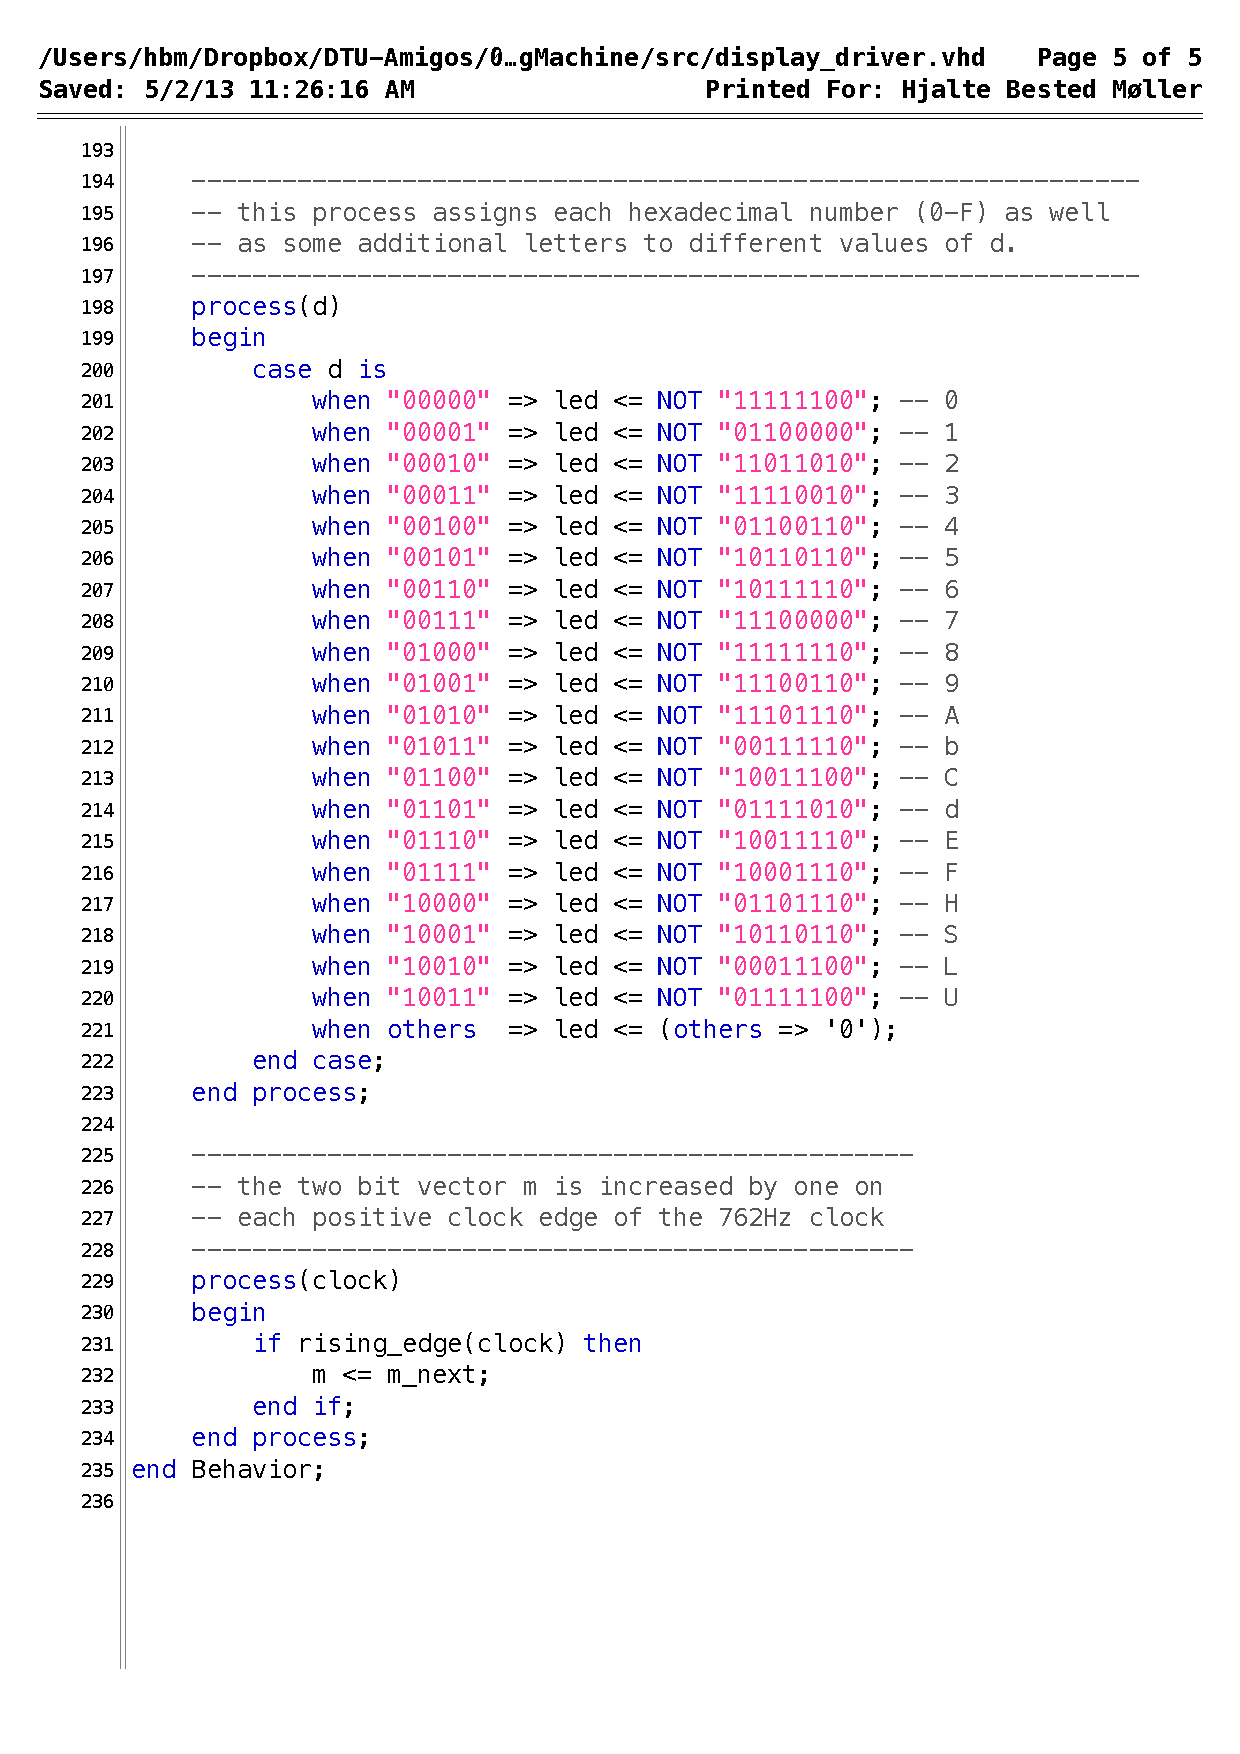
\includegraphics[scale=0.7]{figs/display_driver_5.pdf}
\caption{Page 5}
\label{vhd:dispdriv5}
\end{figure}

%DISPLAY DRIVER END

%INPUT SYNCHRONIZER

\begin{figure}[!h]
\centering
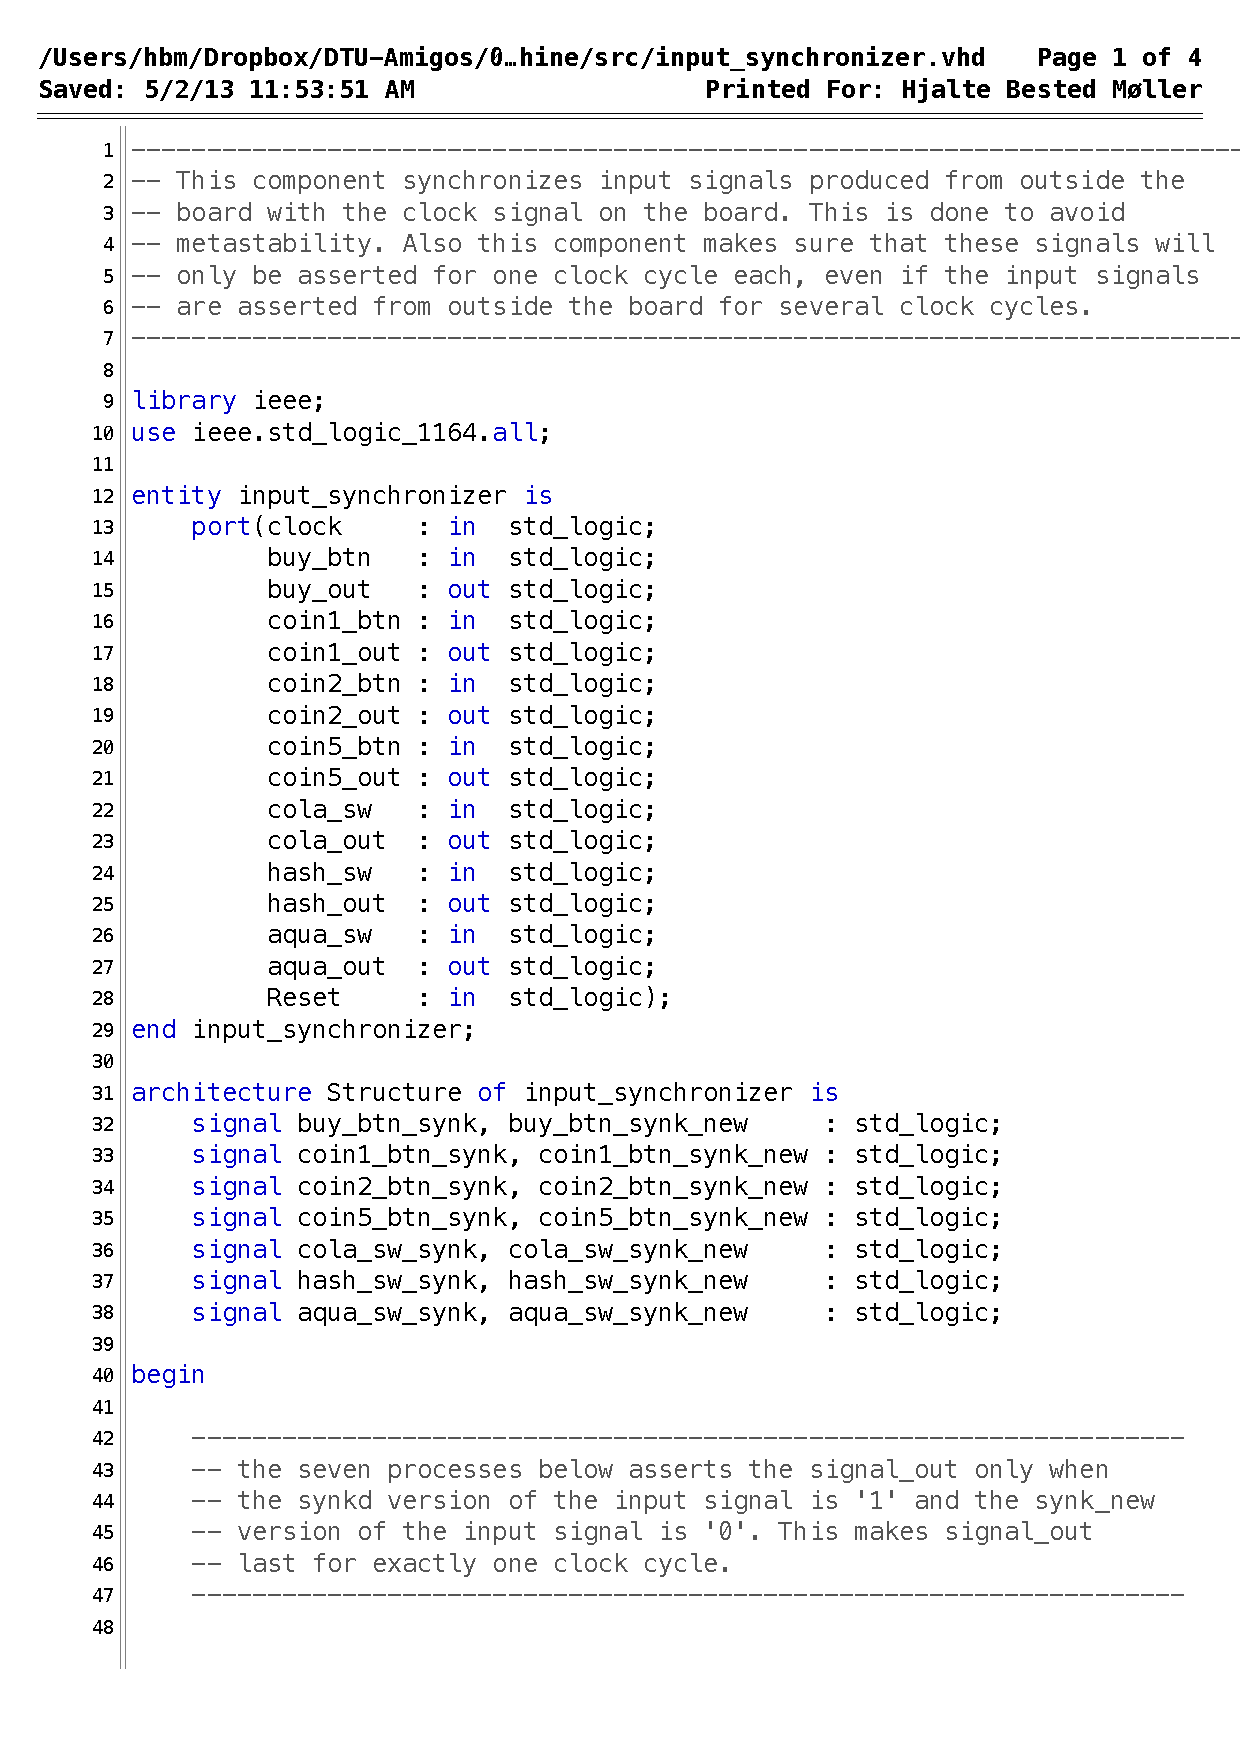
\includegraphics[scale=0.6]{figs/input_synchronizer.pdf}
\caption{VHDL code for the input synchronizer which synchronizes the input signals to the clock}
\label{vhd:inpsync1}
\end{figure}

\begin{figure}[!h]
\centering
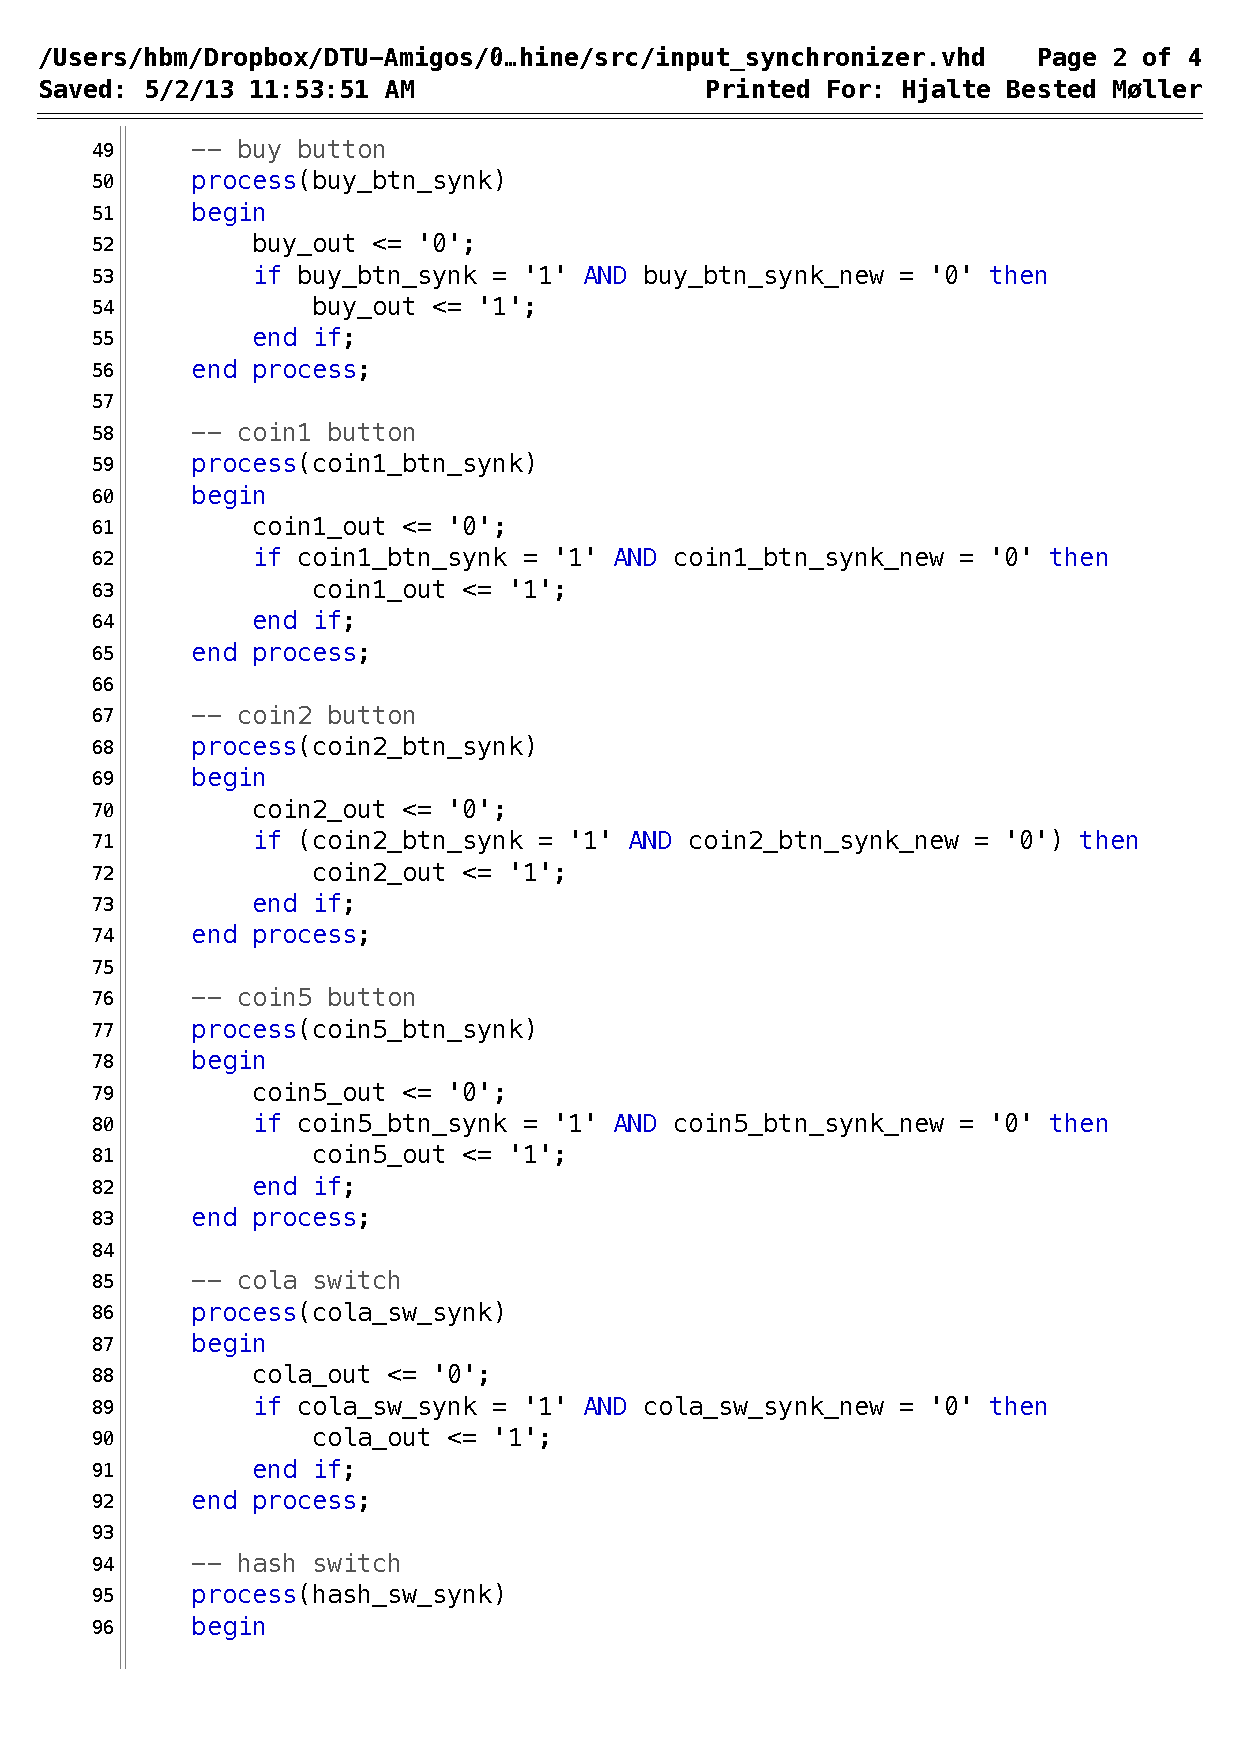
\includegraphics[scale=0.6]{figs/input_synchronizer_2.pdf}
\caption{Page 2}
\label{vhd:inpsync2}
\end{figure}

\begin{figure}[!h]
\centering
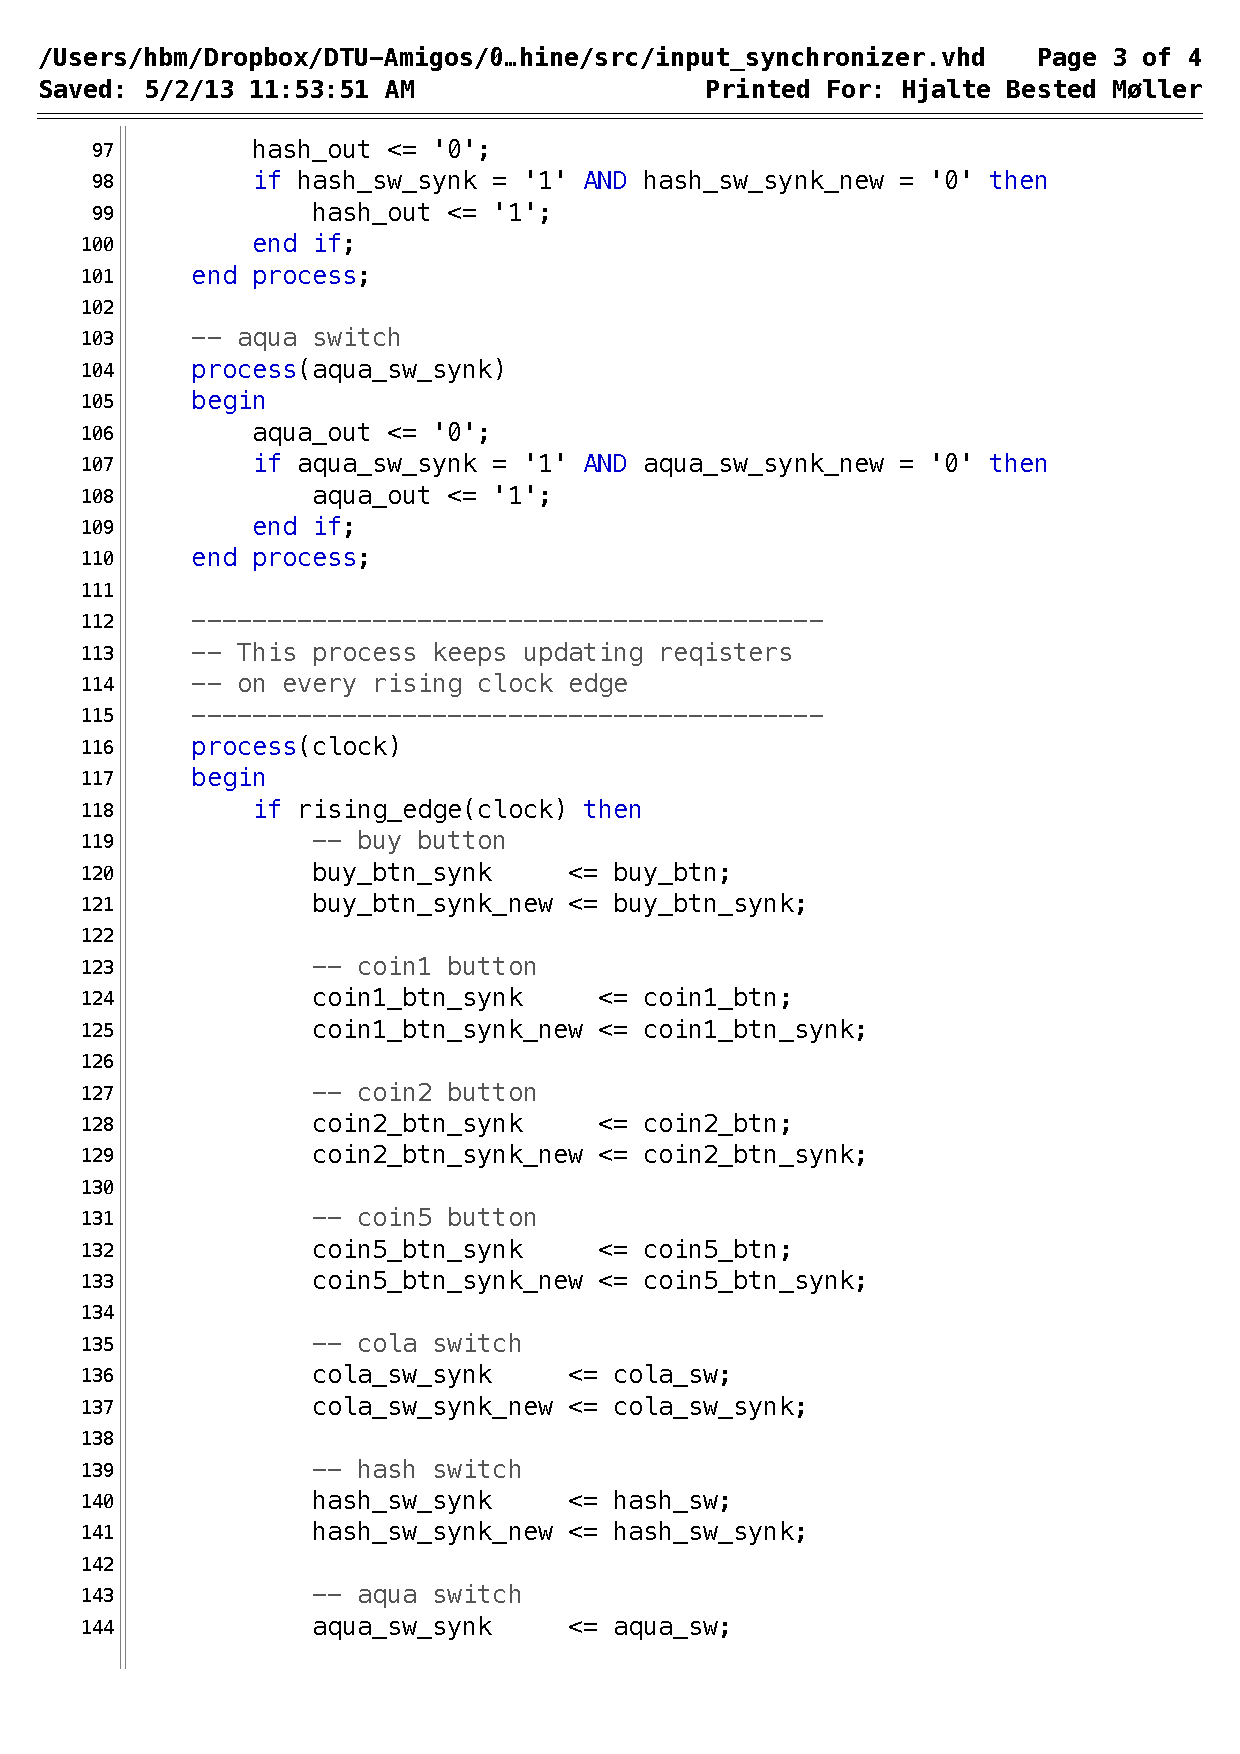
\includegraphics[scale=0.6]{figs/input_synchronizer_3.pdf}
\caption{Page 3}
\label{vhd:inpsync3}
\end{figure}

\begin{figure}[!h]
\centering
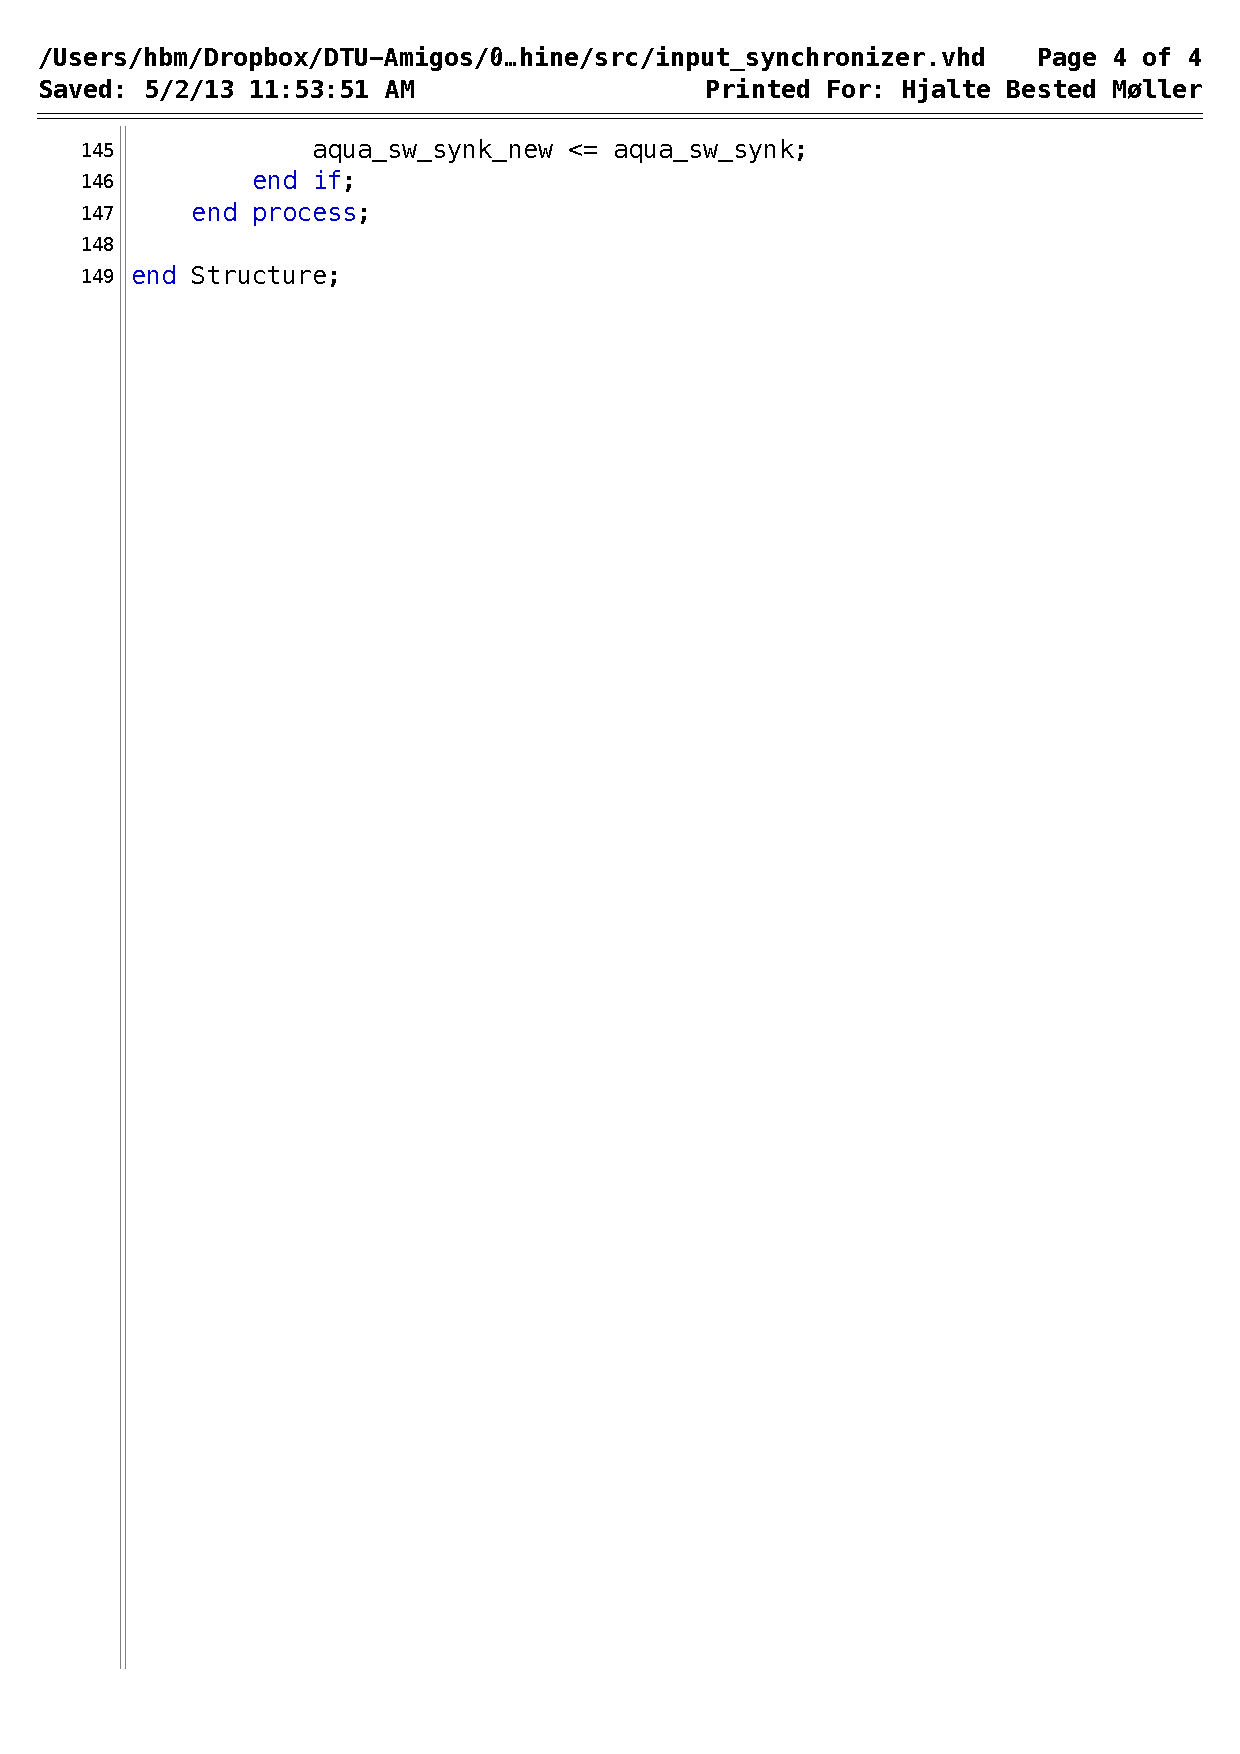
\includegraphics[scale=0.6]{figs/input_synchronizer_4.pdf}
\caption{Page 4}
\label{vhd:inpsync4}
\end{figure}

%INPUT SYNCHRONIZER END

%PROCESSING UNIT

\begin{figure}[!h]
\centering
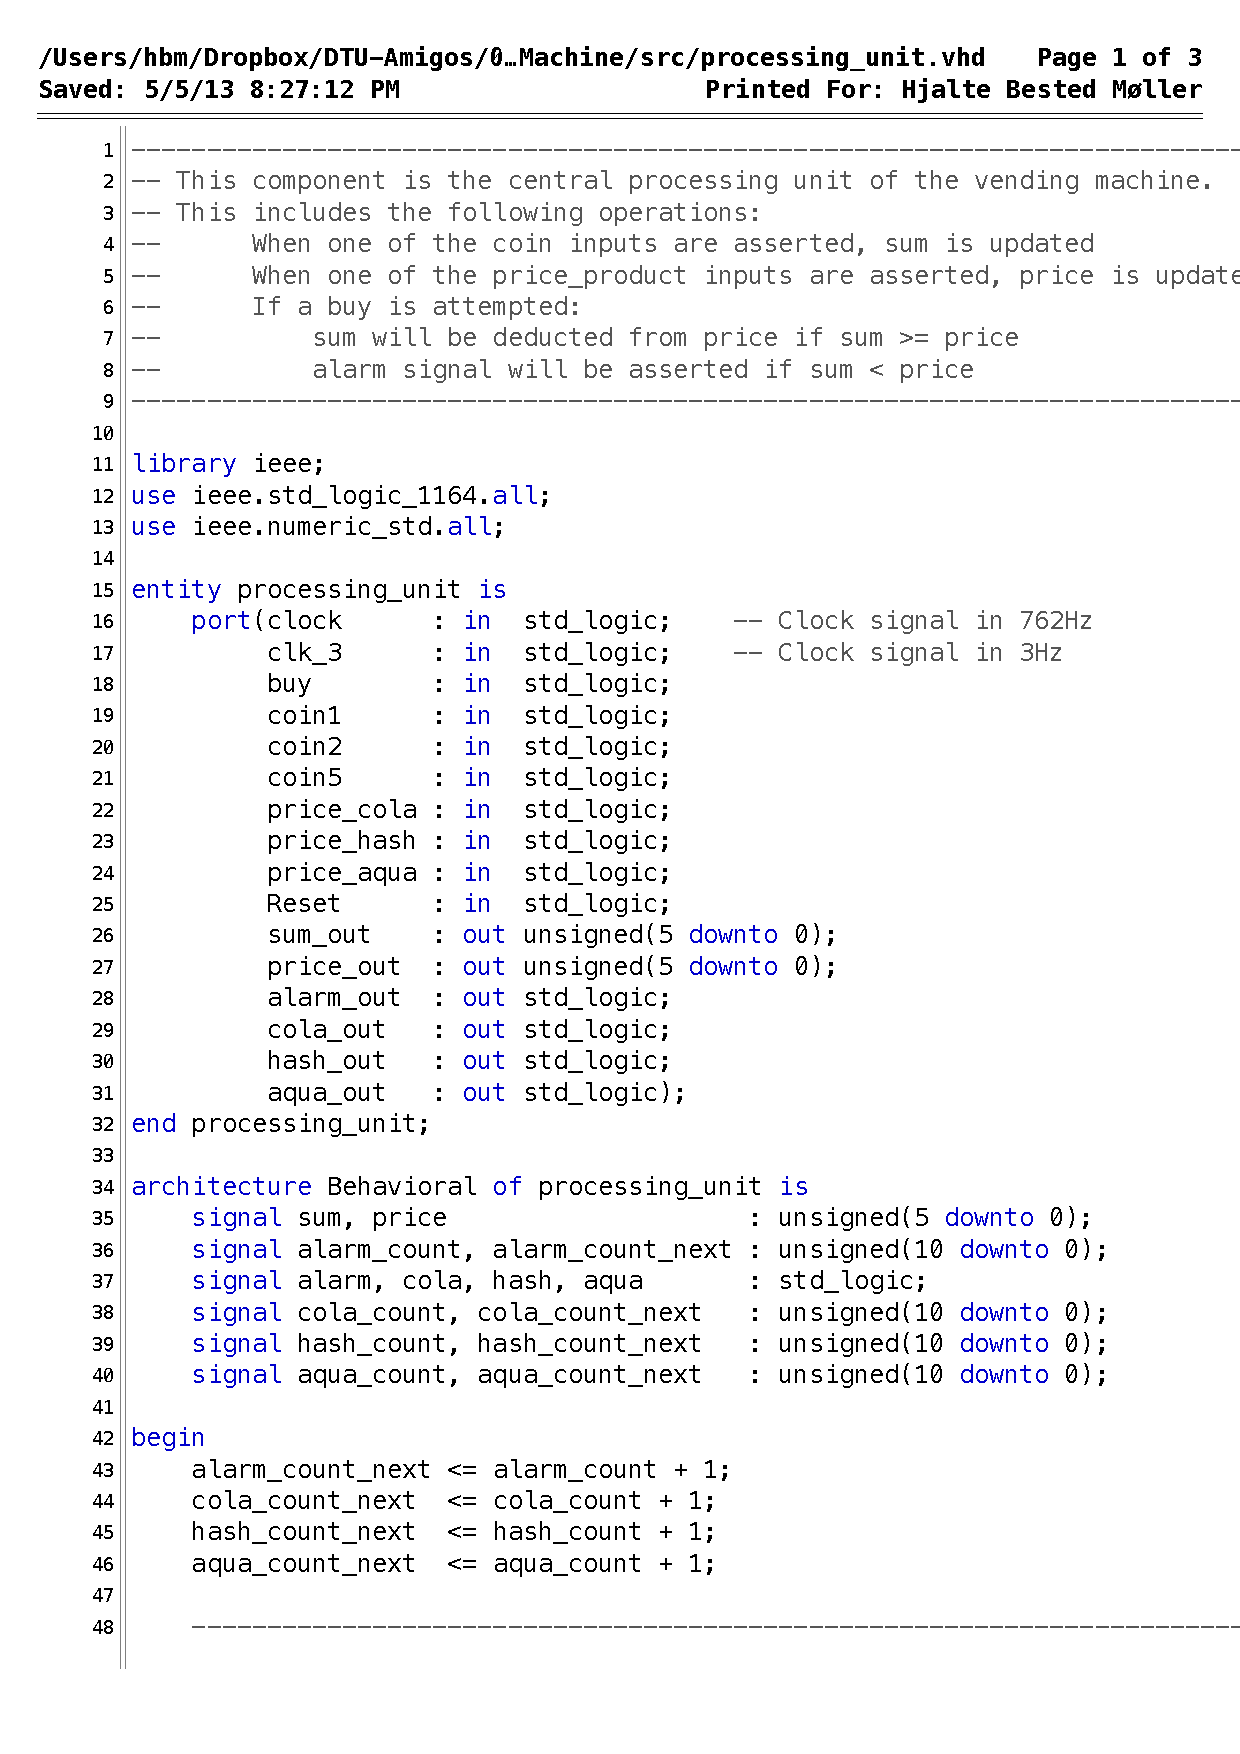
\includegraphics[scale=0.6]{figs/processing_unit.pdf}
\caption{Processing unit, for calculating/setting price/sum}
\label{vhd:proceunit1}
\end{figure}

\begin{figure}[!h]
\centering
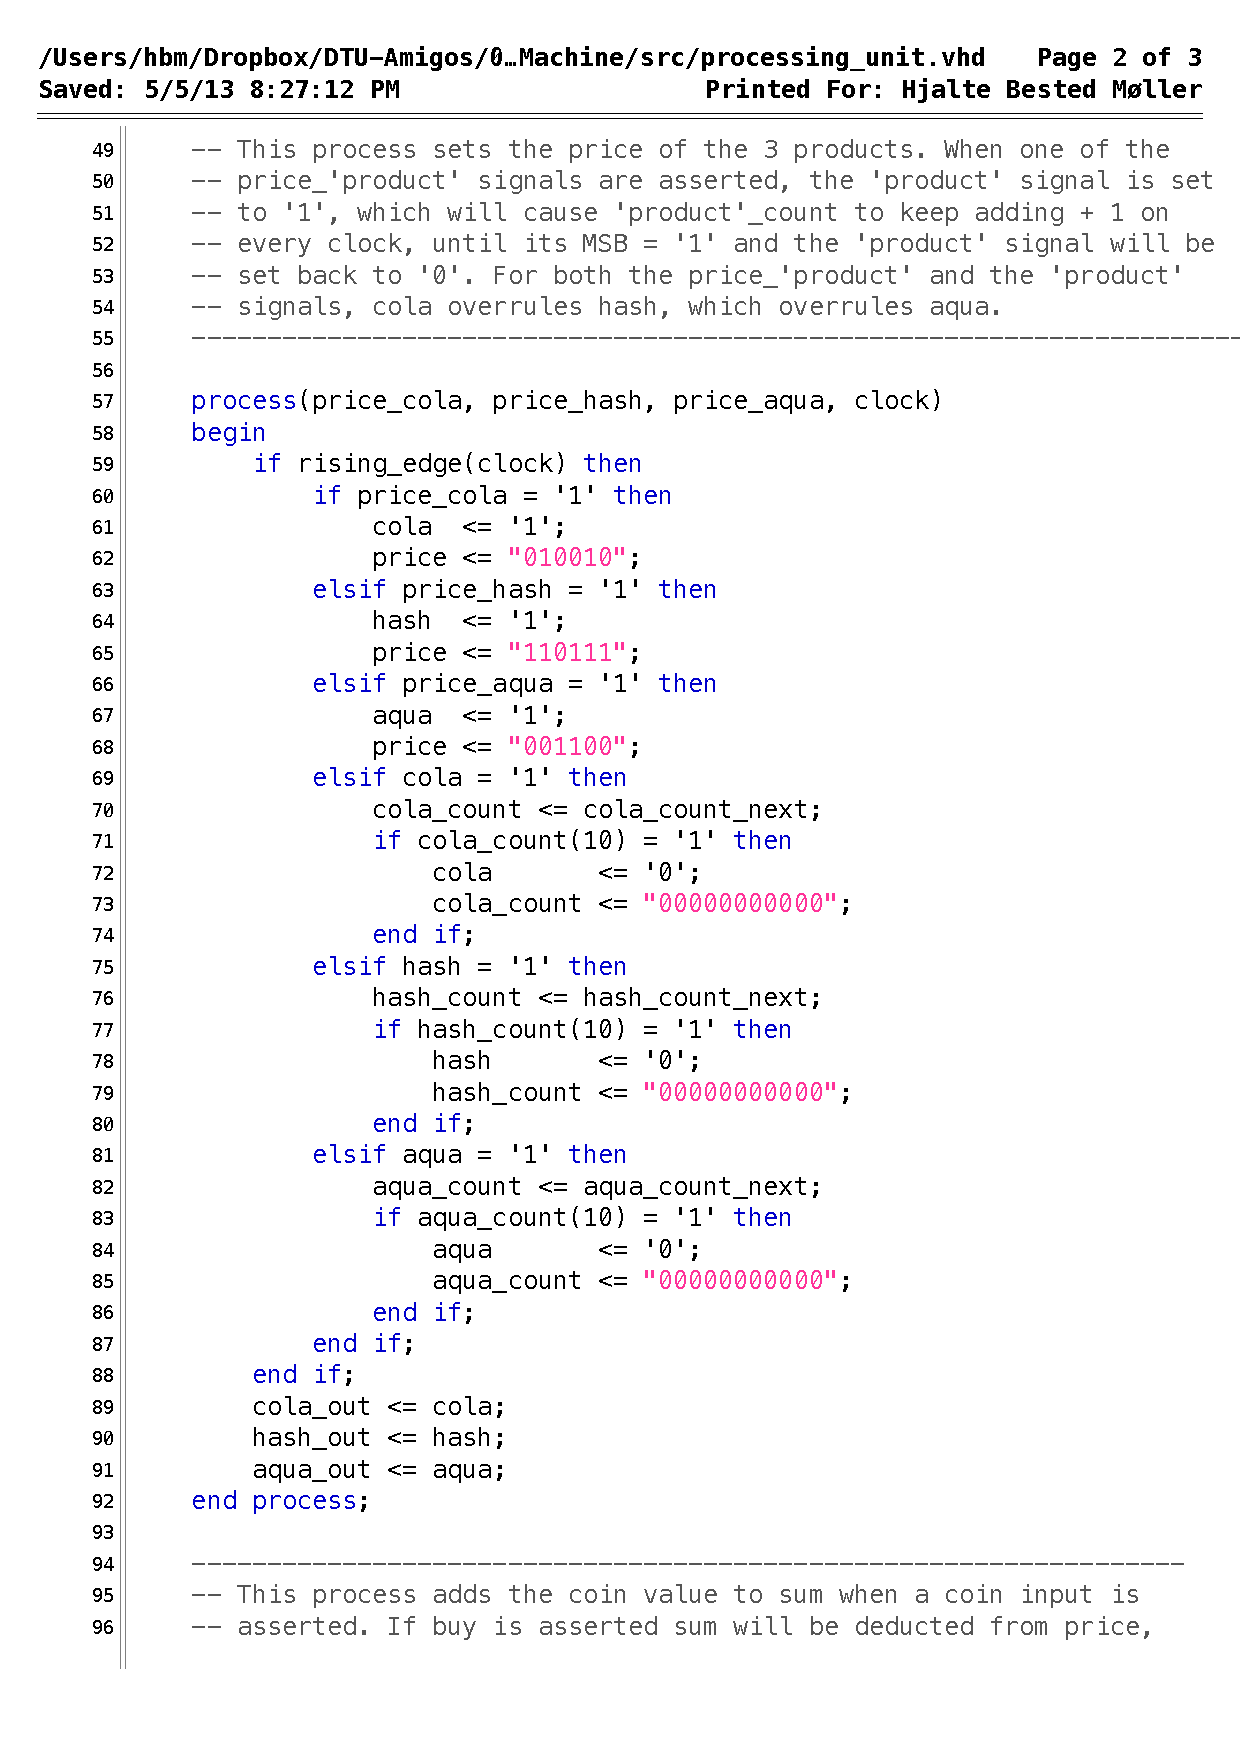
\includegraphics[scale=0.6]{figs/processing_unit_2.pdf}
\caption{Page 2}
\label{vhd:proceunit2}
\end{figure}

\begin{figure}[!h]
\centering
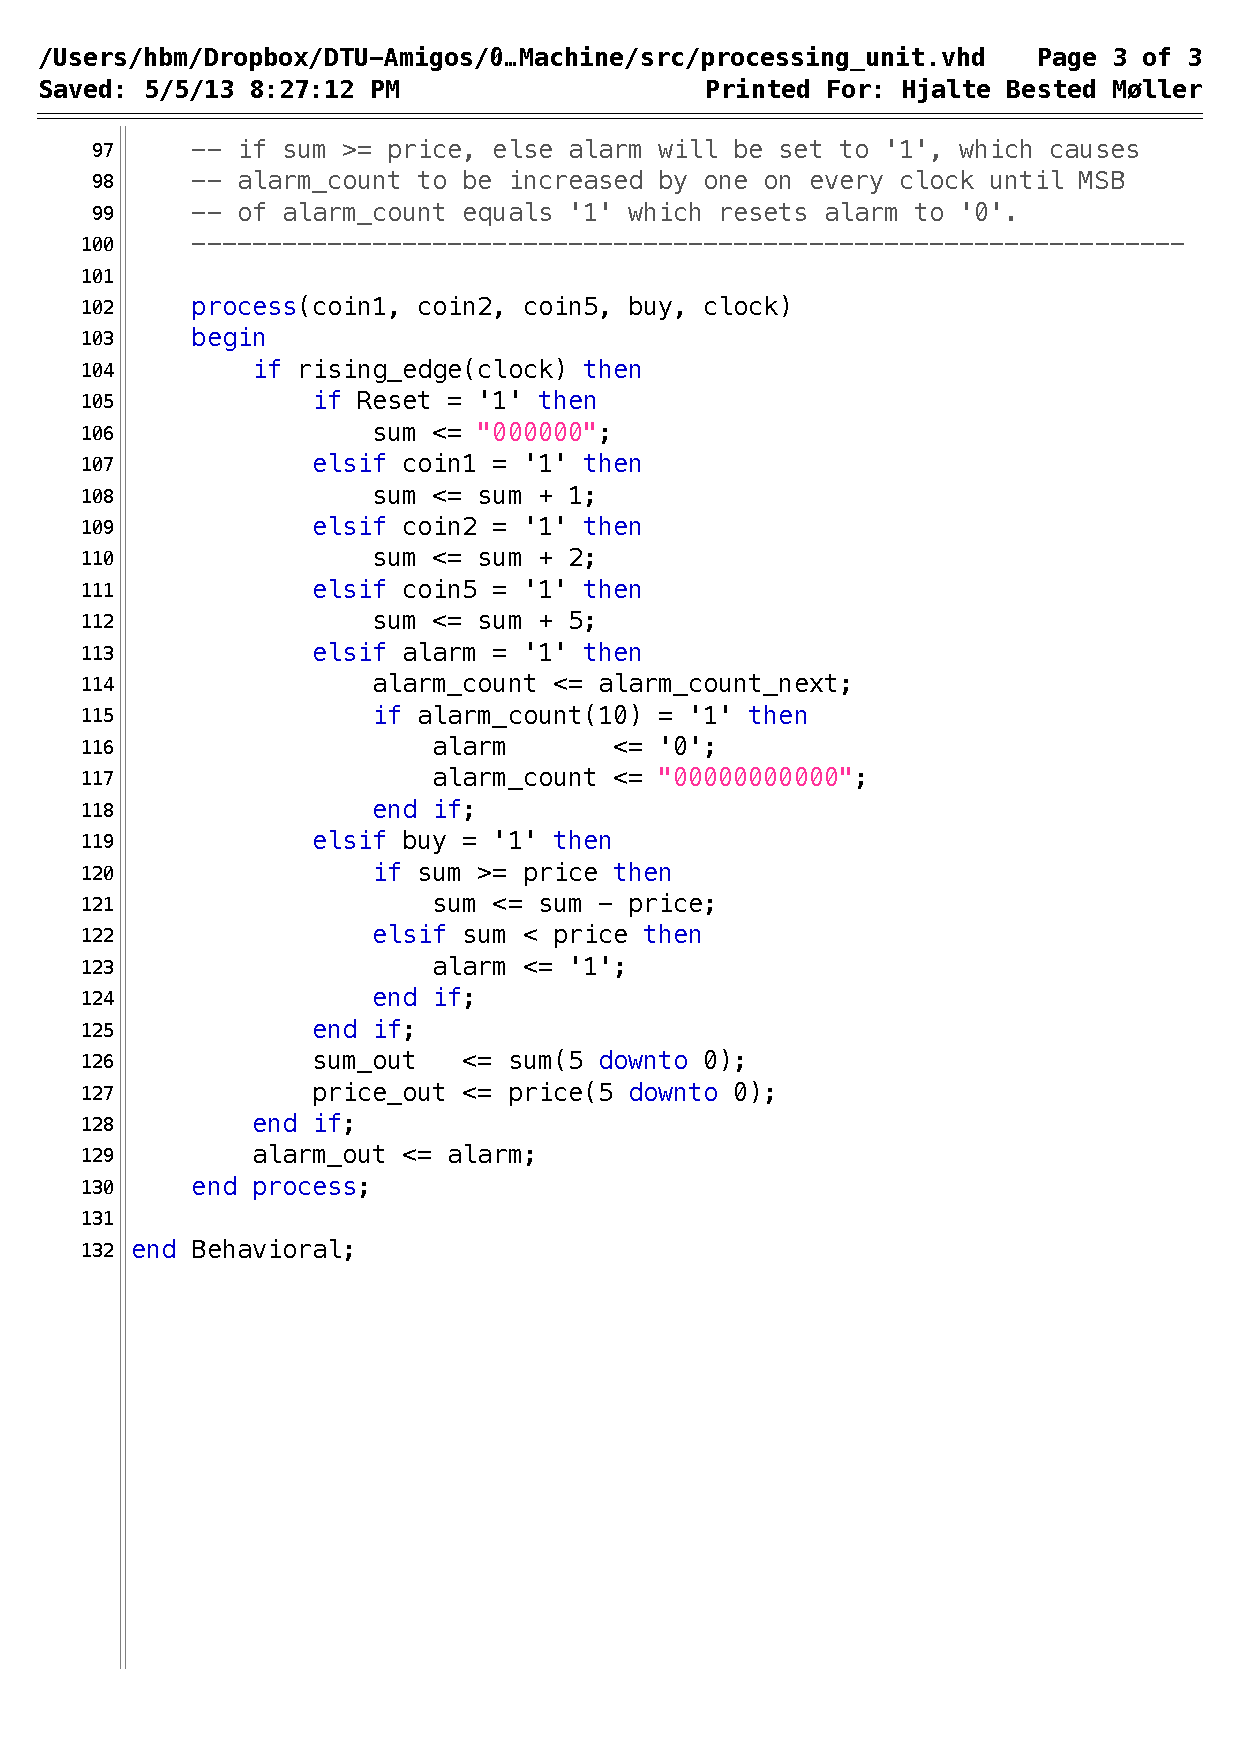
\includegraphics[scale=0.6]{figs/processing_unit_3.pdf}
\caption{Page 3}
\label{vhd:proceunit3}
\end{figure}

%PROCESSING UNIT END

%VENDING MACHINE

\begin{figure}[!h]
\centering
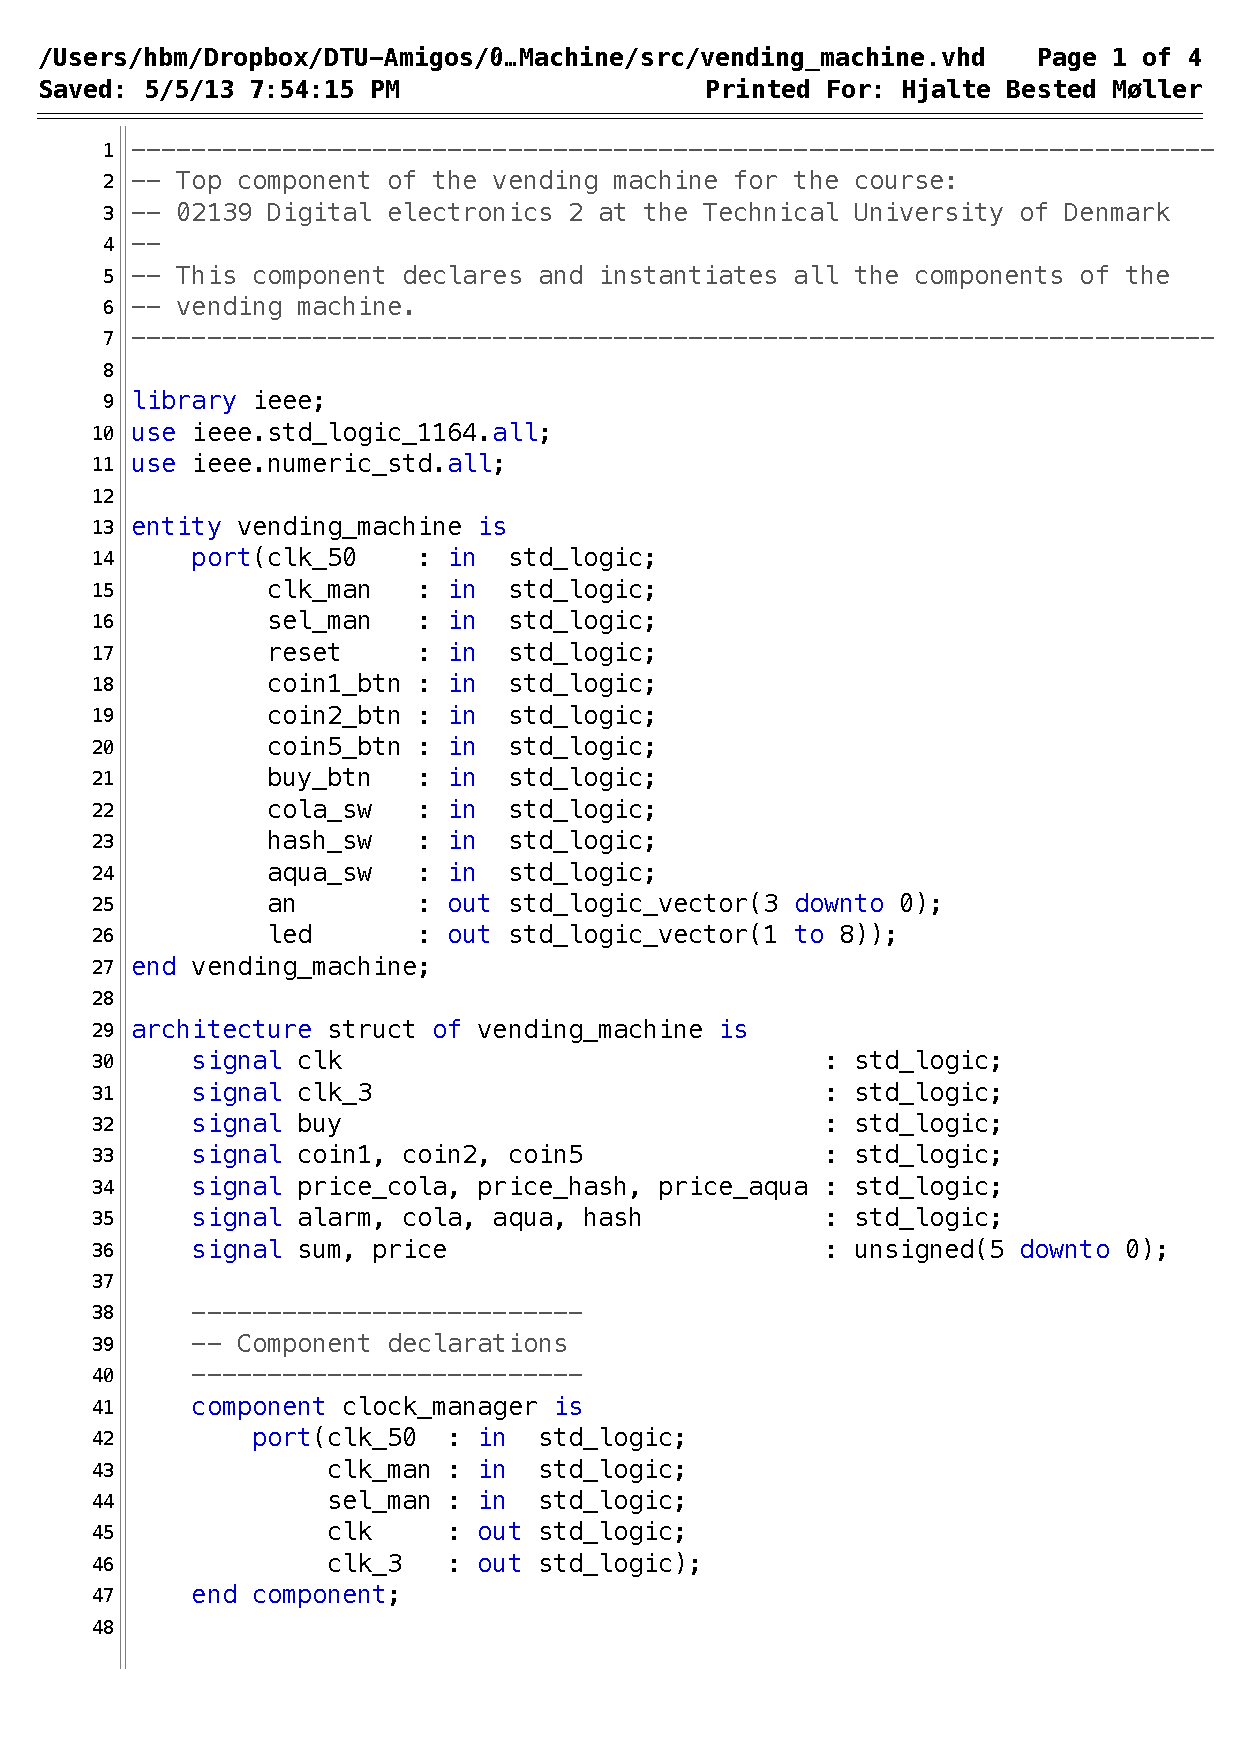
\includegraphics[scale=0.6]{figs/vending_machine.pdf}
\caption{The complete vending machine, assembling all the components}
\label{vhd:vending1}
\end{figure}

\begin{figure}[!h]
\centering
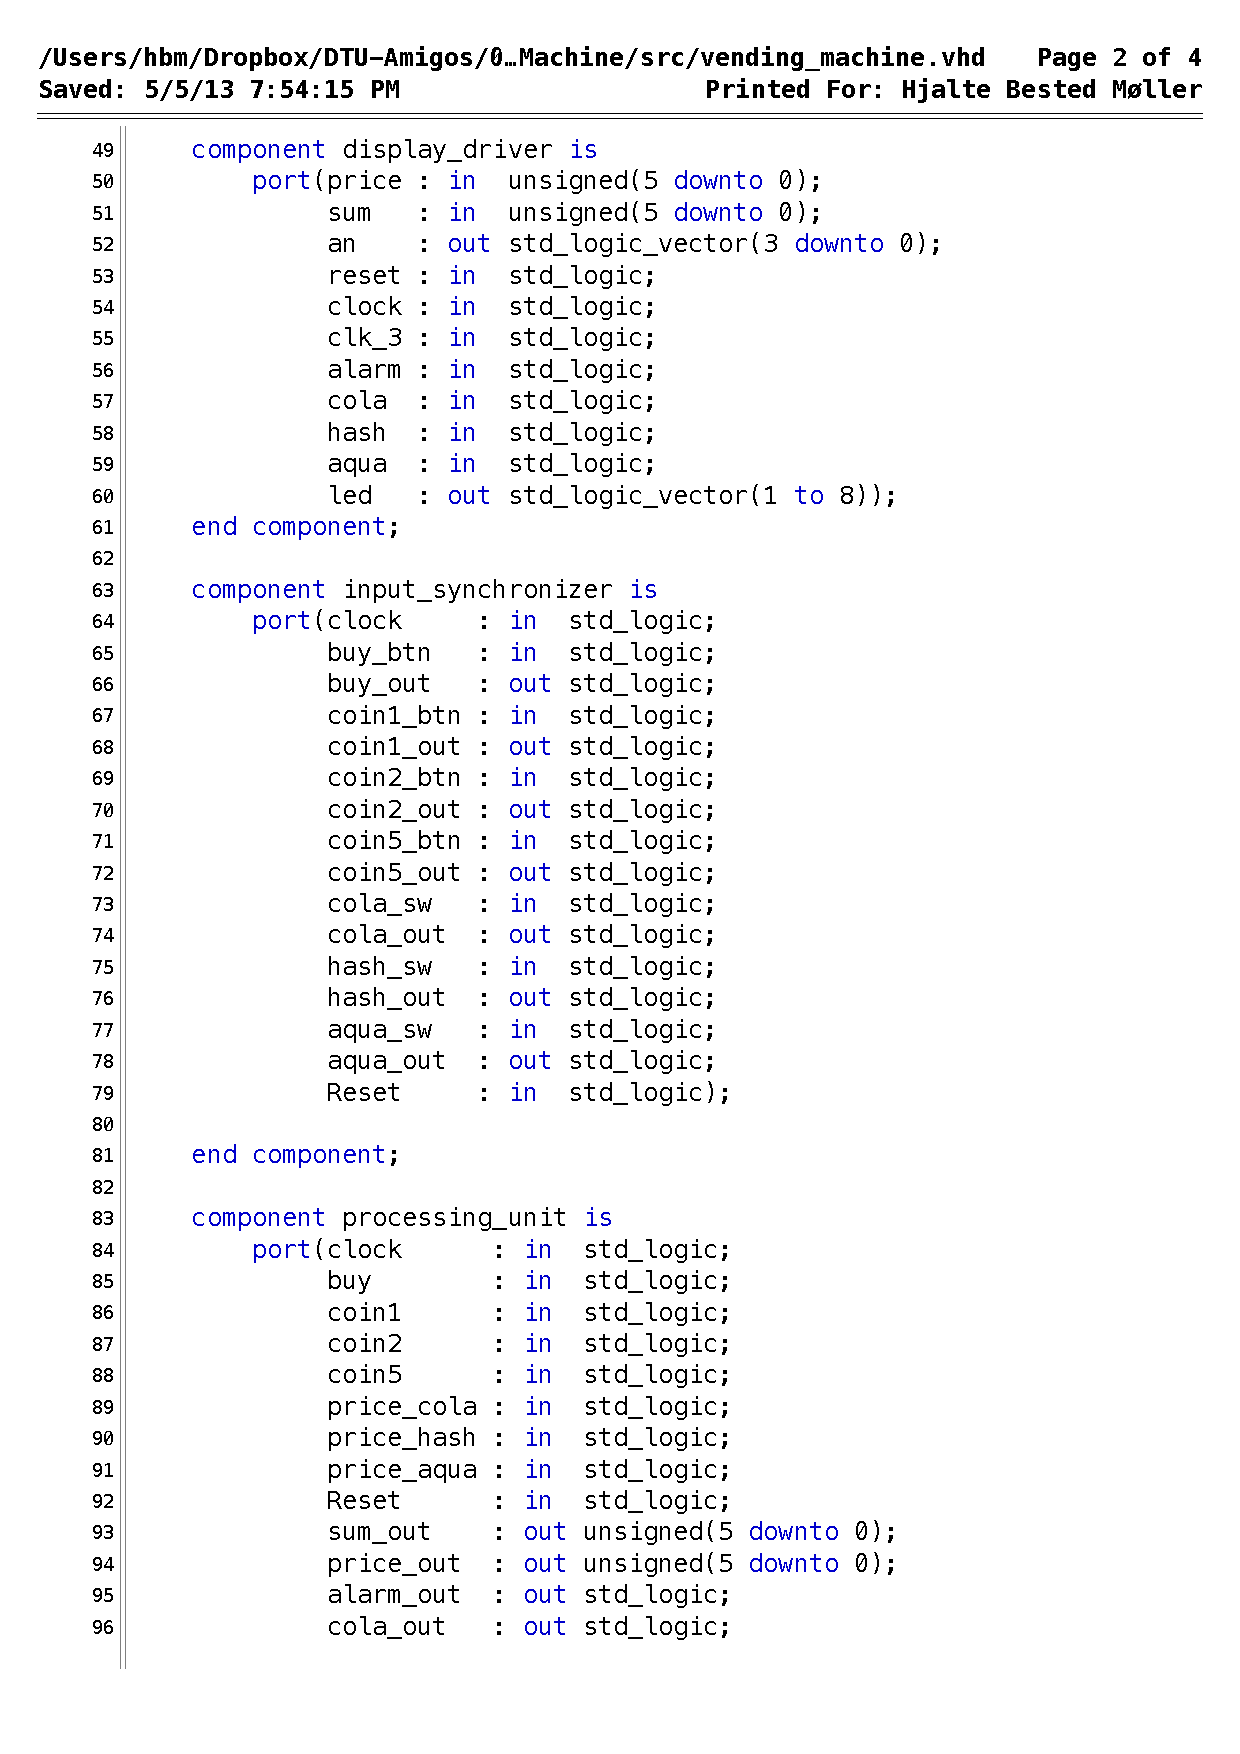
\includegraphics[scale=0.6]{figs/vending_machine_2.pdf}
\caption{Page 2}
\label{vhd:vending2}
\end{figure}

\begin{figure}[!h]
\centering
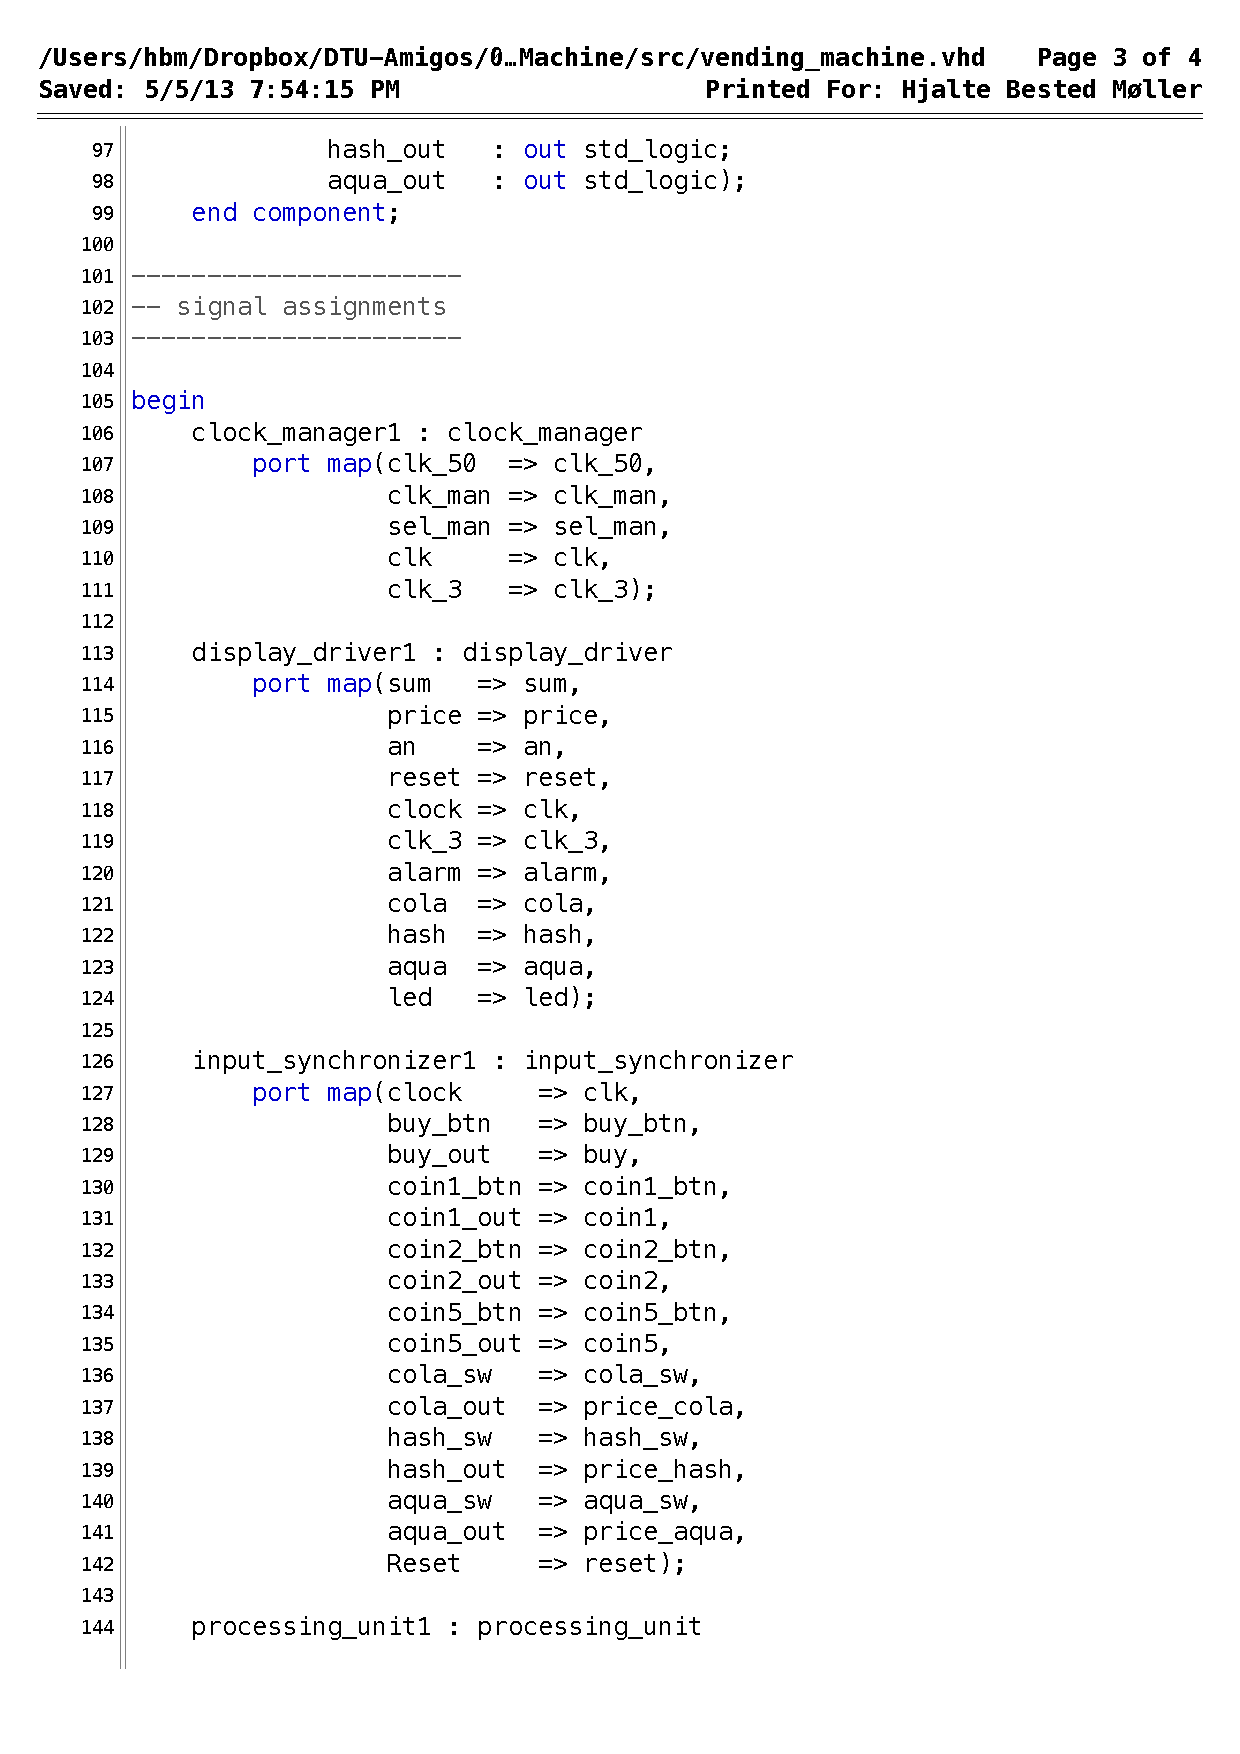
\includegraphics[scale=0.6]{figs/vending_machine_3.pdf}
\caption{Page 3}
\label{vhd:vending3}
\end{figure}

\begin{figure}[!h]
\centering
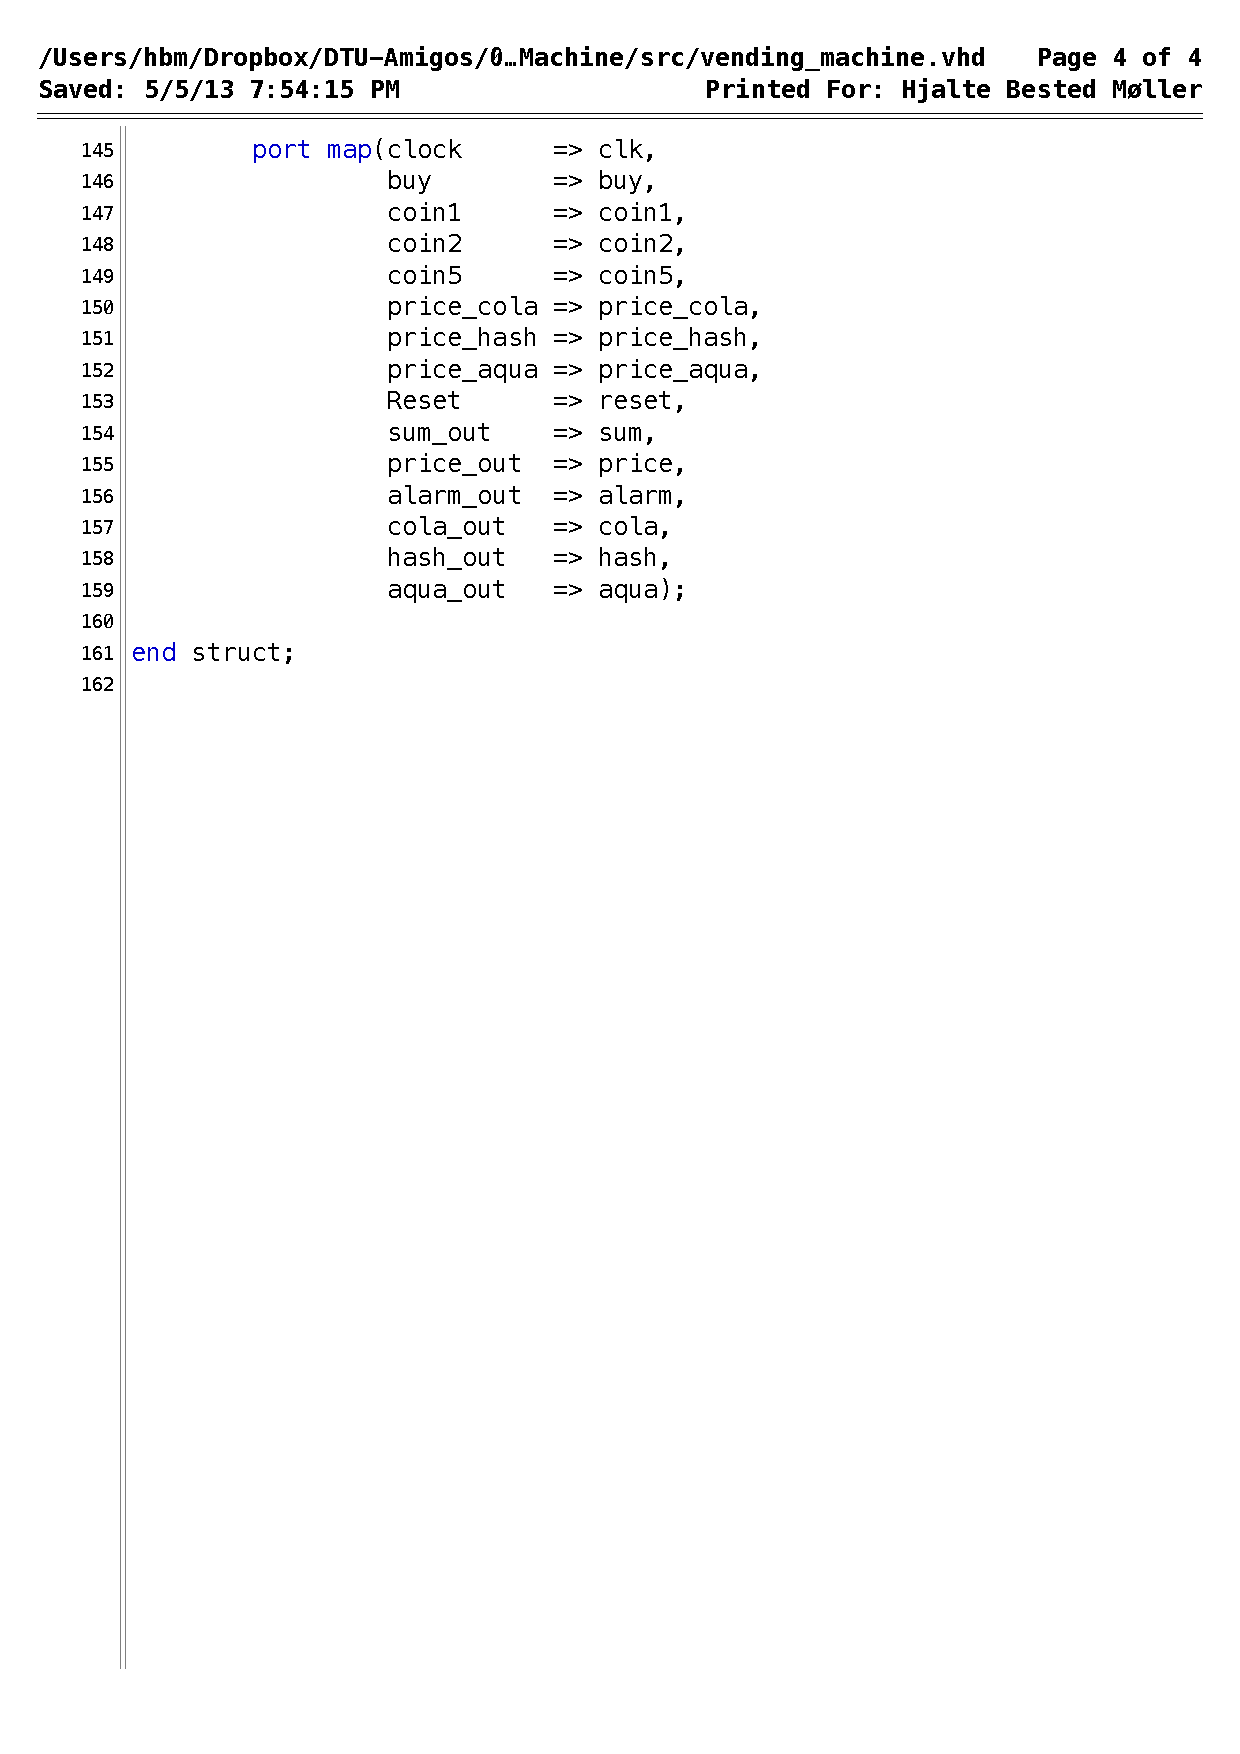
\includegraphics[scale=0.6]{figs/vending_machine_4.pdf}
\caption{Page 4}
\label{vhd:vending4}
\end{figure}

%VENDING MACHINE END

%%%%%%%%%%%%%%%%%%%%%%%%
%%% THE BIBLIOGRAPHY %%%
%%%%%%%%%%%%%%%%%%%%%%%%

		
	
		
\end{document}
